\documentclass[conference]{IEEEtran}
\IEEEoverridecommandlockouts

% The preceding line is only needed to identify funding in the first footnote. If that is unneeded, please comment it out.
\usepackage{cite}
\usepackage{amsmath,amssymb,amsfonts}
\usepackage{algorithmic}
\usepackage{graphicx}
\usepackage{textcomp}
\usepackage{xcolor}
\usepackage{multirow}
\usepackage{amsthm}
\usepackage{mathrsfs}
\usepackage{manyfoot}
\usepackage{booktabs}
\usepackage{algorithm}
\usepackage{listings}
\usepackage{times}
\usepackage{epsfig}
\usepackage[export]{adjustbox}
\usepackage{tabularx}
\usepackage{xurl}
\usepackage[hidelinks,breaklinks=true]{hyperref}
\Urlmuskip=0mu plus 1mu

\def\BibTeX{{\rm B\kern-.05em{\sc i\kern-.025em b}\kern-.08em
    T\kern-.1667em\lower.7ex\hbox{E}\kern-.125emX}}

\begin{document}

\title{AGI-Former: a novel and testable end-to-end deep learning model for artificial general intelligence\\
%{\footnotesize \textsuperscript{*}Note: Sub-titles are not captured in Xplore and
%should not be used}
%\thanks{Identify applicable funding agency here. If none, delete this.}
}

\author{
\IEEEauthorblockN{Zanyar Zohourianshahzadi}
\IEEEauthorblockA{
\textit{Artificial Intelligence, Computer Science, and CyberSecurity} \\
\textit{B.S. CS \& IT: Azad University of Tehran South Branch} \\
\textit{M.S. IT \& CyberSecurity: Colorado Technical University} \\
\textit{Ph.D. AI \& CS: University of Colorado Colorado Springs} \\
Colorado Springs, Colorado, USA \\
Email: {zanyarz@me.com \& zanyarz@gmail.com}
}
}

\maketitle

\begin{abstract}
Artificial general intelligence (AGI) requires more than placing specialist models behind a shared interface. It requires an integrated architecture that transforms heterogeneous observations into persistent state, coherent reasoning, and grounded action. This paper introduces AGI-Former, a novel and testable end-to-end deep learning architecture for AGI formulated as integrated multimodal agency. AGI-Former combines modality-specific encoders for language, images, video, audio, and extensible sensory streams with a causal thought-action decoder and Unified Attention mechanisms derived from the Unified Transformer (UTR). Three complementary configurations are developed. The disjoint architecture produces specialized output streams for distinct modalities, tools, effectors, or regions. The joint architecture performs action-conditioned multimodal fusion and generates a unified thought-action sequence. The hierarchical architecture combines joint global coordination with disjoint regional execution through recurrent supervisory, state, action, uncertainty, and feedback tokens. To make the proposal falsifiable, we specify matched-budget baselines, mechanism-level ablations, held-out generalization tests, causal grounding interventions, robustness evaluations, coordination measures, and efficiency metrics. We identify the absence of coherent datasets linking synchronized multimodal observations, state, reasoning, actions, consequences, and feedback as the primary practical limitation, alongside training cost. Scientifically rich videos and embodied datasets are proposed as starting points for constructing bounded training episodes and progressively scaled experiments. AGI-Former is presented not as evidence that AGI has been achieved, but as an implementable and empirically testable architecture for investigating integrated multimodal agency.
\end{abstract}

\begin{IEEEkeywords}
Super Intelligence, AGI, General Intelligence, Artificial Consciousness, Machine Consciousness
\end{IEEEkeywords}


\section{\textbf{Introduction}}

The Transformer was introduced as a complete encoder--decoder architecture for sequence transduction \cite{vaswani2017attention}. Its encoder constructs contextual representations of an input sequence, while its decoder combines a causal output state with encoder information to generate a conditional sequence. Subsequent progress has produced highly capable but increasingly specialized families. Encoder-oriented models such as BERT emphasize bidirectional representation learning \cite{devlin2019bert}; Vision Transformers apply encoder-style processing to image patches \cite{dosovitskiy2021image}; and GPT-style models emphasize causal decoder stacks for autoregressive generation \cite{brown2020language}. These specializations have been productive, but they divide perception, representation, and generation across model families that are not inherently organized as one persistent agent.

Multimodal research has begun to reconnect these capabilities. Flamingo conditions a language model on visual representations through gated cross-attention \cite{alayrac2022flamingo}; PaLM-E injects continuous sensor representations into an embodied language model \cite{driess2023palme}; Perceiver IO maps heterogeneous inputs and outputs through a shared latent space \cite{jaegle2022perceiver}; and Gato represents multiple modalities, tasks, embodiments, and action spaces as token sequences processed by one generalist policy \cite{reed2022generalist}. These systems demonstrate that heterogeneous observations and outputs can participate in shared computation. Nevertheless, processing several modalities is not by itself equivalent to an architecture in which multimodal perception, internal thought, and action continuously condition one another.

Commercial AI platforms now reinforce this distinction. Systems such as ChatGPT and Claude expose broad conversational interfaces through which users can analyze text, images, and documents and invoke additional tools or services \cite{openai2026chatgpt,anthropic2026claude}. From the user's perspective, these systems can resemble integrated intelligence because heterogeneous requests enter through one interface and useful responses or actions return through the same interface. However, an end-to-end service is not necessarily an end-to-end neural architecture. Public interfaces do not reveal the complete internal architectures of proprietary systems, and this paper therefore makes no claim about their undisclosed implementations. What can be observed more generally is a system-level design pattern in which language models coordinate modality-specific models, retrieval components, tools, and execution environments. HuggingGPT provides a published example: a language model plans a task, selects expert models, executes the selected models, and summarizes their outputs across language, vision, and speech tasks \cite{shen2023hugginggpt}.

This orchestration pattern is powerful and immediately practical, but it introduces a distinction among three levels of integration. \textit{Interface integration} presents multiple capabilities through one interaction surface. \textit{System integration} connects models and tools through software, routing rules, intermediate representations, and execution logic. \textit{Architectural integration} learns the relationships among perception, internal state, and action within a jointly trainable neural architecture. The first two levels can provide broad functionality, yet architectures of this class may require model selection, data conversion, prompt construction, communication among components, and separate deployment and maintenance paths. These operations can add engineering complexity, latency, and computational overhead. They can also prevent errors originating in an early specialist or textual conversion from being corrected through direct end-to-end learning. This observation does not diminish modular systems; it motivates a complementary question: can more of the integration currently achieved by external orchestration be learned within one architecture?

Our preceding work provides the conceptual path to this question. Intelligence was defined operationally as information-dependent selection among possible actions, states, or outputs, while remaining distinct from phenomenal consciousness \cite{zohourian2026intelligence}. Artificial consciousness was then considered in multiple possible forms, with language proposed as a unifying interface through which heterogeneous artificial minds can communicate without requiring identical internal representations \cite{zohourian2026language}. We subsequently distinguished artificial general intelligence from consciousness and characterized AGI as integrated multimodal agency: the coordination of perception, memory, objectives, reasoning, planning, and action across modalities, tasks, and environments \cite{zohourian2026agi}. Finally, we separated general intelligence from superintelligence, defining the latter through machine capabilities that extend the frontier of knowledge by discovery, fusion, or invention rather than merely reproducing or accelerating known procedures \cite{zohourian2026superintelligence}. Together, these arguments identify integrated agency as an architectural problem that precedes claims of either consciousness or superintelligence.

This paper introduces \textit{AGI-Former}, a novel and testable end-to-end deep learning architecture designed to support artificial general intelligence as integrated multimodal agency. AGI-Former directly connects modality-specific perception encoders with causal thought and action generation. Image, video, audio, language, and additional sensory streams are encoded in forms appropriate to their native structure; a decoder state formed from prior thought and action tokens then queries and combines the encoded evidence to generate subsequent thought or action tokens. In this end-to-end mapping, multimodal observations and prior thought or action tokens jointly condition the next thought or action tokens.

The phrase \textit{architecture for AGI} is used deliberately but conservatively. AGI-Former is intended to operationalize the architectural requirements of integrated multimodal agency; it does not imply that any untrained instantiation is generally intelligent, that multimodality alone is sufficient for AGI, or that the architecture establishes consciousness. Its claim is instead scientific and falsifiable: the proposed organization can be implemented, trained, ablated, and compared against modular and partially integrated alternatives using measurable perception, reasoning, coordination, transfer, and action outcomes.

AGI-Former includes an evolutionary baseline as well as the proposed joint architecture. In the baseline organization, image--text, video--text, audio--text, and other modality-to-language specialists convert observations into descriptions that are supplied to a large language model supervisor. The supervisor integrates these descriptions and produces plans, tool calls, or actions. This disjoint organization is compatible with existing components and demonstrates the value of language as an interoperability layer. However, it also makes explicit the limitations of text-mediated integration: modality-native detail can be compressed before joint reasoning begins, specialist errors can propagate forward, and perception cannot be optimized directly against the final action unless gradients and training signals cross the complete pipeline.

The joint AGI-Former architecture removes this required textual bottleneck. Modality-specific encoders preserve the structure of each sensory stream while making their encoded representations directly available to a shared decoder-side thought--action state. The decoder does not merely receive descriptions of observations; it learns which portions of each encoded stream are relevant to the current state and how the selected evidence should affect the next decision. This organization follows the broader principle that multimodal learning depends not only on representation but also on when and how information is aligned and fused \cite{baltrusaitis2019multimodal}.

AGI-Former builds technically upon Unified Attention for Image Classification and Captioning (UTR) \cite{zohourian2026utr}. UTR treats encoding and conditional generation as related attention problems and develops unified attention operations for interactions within and between information streams. AGI-Former extends this foundation from vision--language learning to multimodal agency. The essential transition is from mapping an encoded modality to a descriptive sequence toward mapping several encoded modalities and an evolving causal state to thoughts and actions capable of affecting an environment.

Figure~\ref{fig:transformer_transition} motivates this transition. Rather than treating encoder-only and decoder-only Transformer families as unrelated endpoints, AGI-Former returns to the complete encoder--decoder relation as the fundamental computational unit. Encoders construct representations of what the agent observes; decoder tokens represent what the agent has thought or done; and cross-attention determines which encoded information should condition what the agent thinks or does next. Modality-specific tokenization remains necessary, but the relationship between perception and action is shared and jointly trainable.

\begin{figure*}[t]
    \centering
    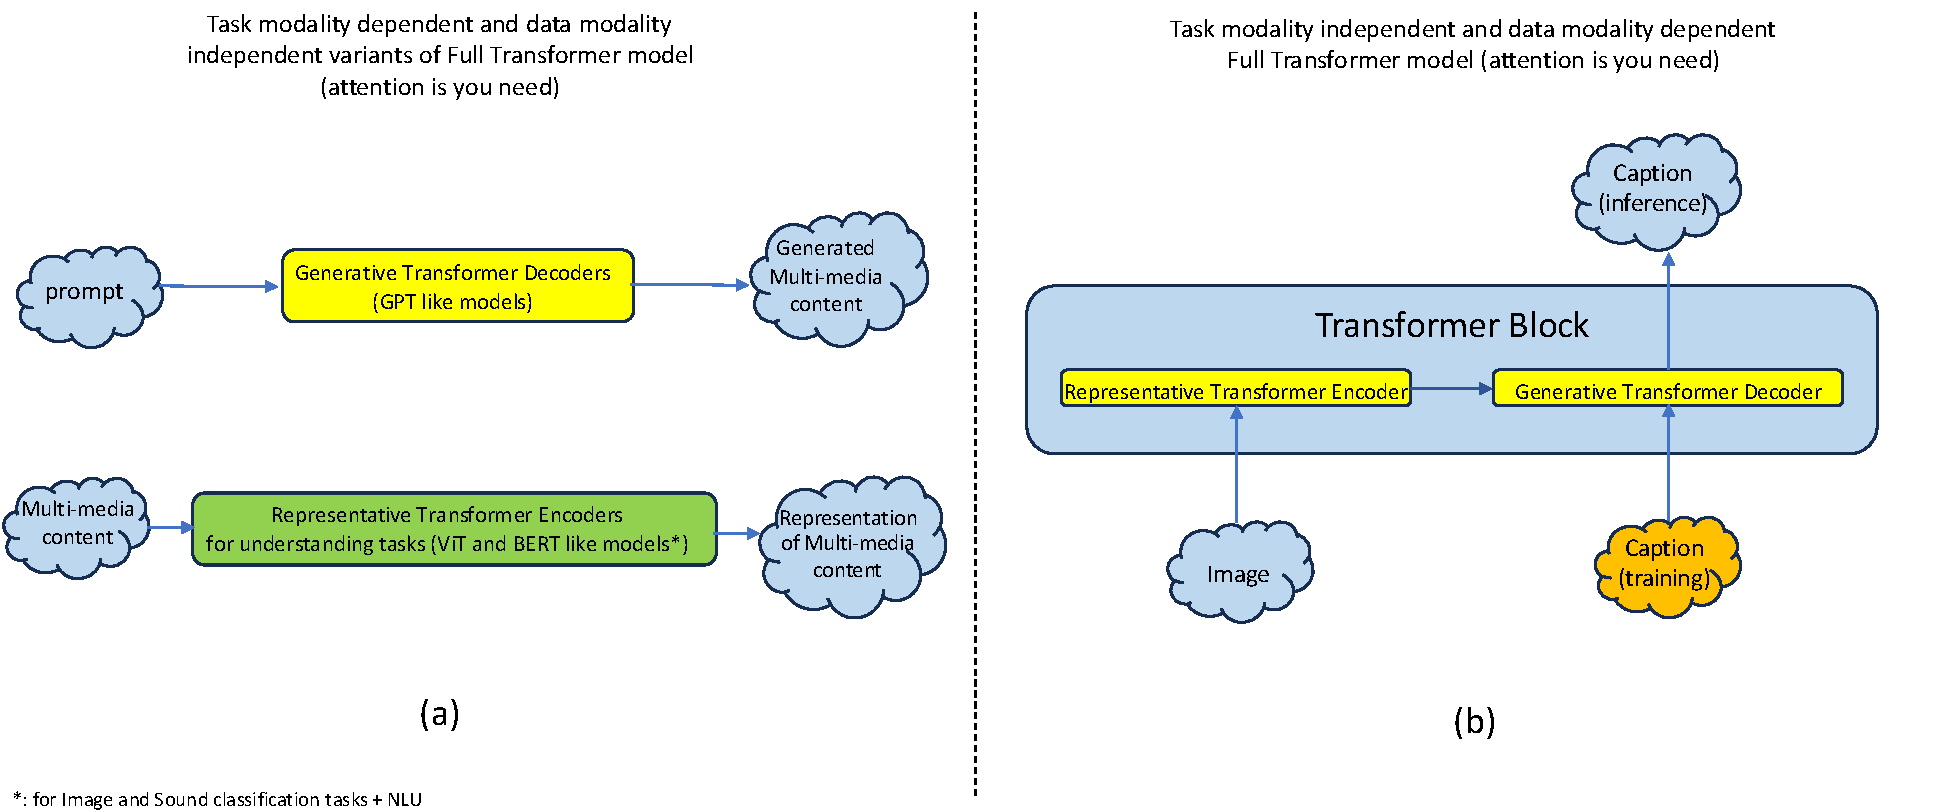
\includegraphics[width=\textwidth]{Figures/fig1.pdf}
    \caption{Conceptual transition from specialized Transformer components to a complete encoder--decoder organization for multimodal perception and conditional thought or action generation.}
    \label{fig:transformer_transition}
\end{figure*}

The proposed framework contains two complementary output organizations. The first generates disjoint modality-conditioned action-token streams. A shared causal thought--action state attends to each encoded modality independently, preserving distinct output spaces or execution requirements when a task demands them. The second generates a joint action-token stream. Each modality is first conditioned on the current thought--action state; the resulting task-relevant representations are then concatenated and used to synthesize one coordinated output. This ordering implements action-conditioned late fusion: the architecture selects relevant evidence within each modality before integrating that evidence into a common decision.

The central hypothesis of AGI-Former is that artificial general intelligence requires more than access to several modalities or the appearance of integration at an interface. It requires an end-to-end trainable mechanism through which multimodal perception, internal thought, and action can repeatedly condition one another. The principal contributions of this paper are as follows:

\begin{itemize}
    \item We introduce AGI-Former as a testable end-to-end encoder--decoder architecture for integrating multimodal perception with causal thought and action generation.
    \item We distinguish interface-level and system-level integration from architectural integration, positioning existing model-and-tool orchestration as a practical baseline rather than the endpoint of multimodal agency.
    \item We define a disjoint specialist organization in which modality-to-language systems communicate with a language-model supervisor, providing an implementable comparison architecture and an evolutionary path toward joint learning.
    \item We propose modality-specific encoders coupled to a shared decoder-side thought--action state, allowing modality-native evidence to participate directly in conditional generation.
    \item We formulate complementary disjoint-output and joint-output organizations, including action-conditioned late fusion for coordinated multimodal decisions.
    \item We extend the unified-attention direction introduced in UTR from image classification and captioning toward multimodal perception, reasoning, and agency, and define a falsifiable experimental program based on training, ablation, transfer, coordination, and action performance.
\end{itemize}

The remainder of this paper reviews the relevant Transformer, multimodal, and generalist-agent literature; formalizes the input representations and unified attention operations; presents the disjoint and joint AGI-Former architectures; specifies training objectives and evaluation protocols; and concludes with limitations and directions for implementation.

\section{\textbf{Related Work}}

\subsection{\textbf{General Intelligence and Cognitive Architectures}}

Research on general machine intelligence predates contemporary deep learning. Turing shifted the question of whether a machine could think toward an operational test based on observable interaction \cite{turing1950computing}. Later definitions sought to characterize intelligence independently of a particular embodiment or task. Legg and Hutter formalized universal intelligence in terms of an agent's expected performance across computable environments \cite{legg2007universal}, while Goertzel described AGI as the construction of systems possessing broad, general-purpose intelligence rather than competence restricted to a narrow domain \cite{goertzel2014agi}. Chollet subsequently argued that task-specific skill is insufficient as a measure of intelligence and emphasized skill-acquisition efficiency, priors, experience, and generalization to novel problems \cite{chollet2019measure}. These formulations differ in their assumptions and evaluation methods, but collectively move the discussion away from performance on a fixed task and toward adaptive competence across tasks and environments.

Architectural approaches to this goal historically emphasized explicit cognitive organization. Soar proposed an implemented architecture for general intelligent behavior based on problem spaces, goals, production rules, learning, and persistent knowledge \cite{laird1987soar}. ACT-R similarly integrated perceptual--motor processing, goals, declarative memory, production rules, and subsymbolic selection mechanisms within a unified theory of cognition \cite{anderson2004integrated}. These systems established an important principle retained by AGI-Former: general behavior is unlikely to arise from an isolated prediction function without mechanisms that connect perception, memory, internal state, decision, and action. Their integration, however, is primarily constructed through symbolic or hybrid cognitive modules. AGI-Former investigates a different implementation path in which multimodal representations and causal thought--action generation are connected through an end-to-end trainable deep neural architecture.

\subsection{\textbf{Generalist and Multimodal Sequence Models}}

Transformer-based generalist models replace some hand-designed cognitive interfaces with shared sequence modeling. Gato demonstrated that a single network with a common token interface could perform language, image captioning, simulated control, and real-robot tasks \cite{reed2022generalist}. Perceiver IO generalized attention-based processing across structured input and output spaces through a latent representation \cite{jaegle2022perceiver}. Flamingo and PaLM-E showed complementary methods for connecting visual or continuous sensor representations to large language models \cite{alayrac2022flamingo,driess2023palme}. As discussed in Section~I, these works establish that heterogeneous modalities, tasks, and embodiments can share substantial computation. For the present comparison, their most important distinction is architectural: Gato is organized as a generalist sequence policy, Perceiver IO uses a latent input--output interface, and Flamingo and PaLM-E remain centered on language-model computation conditioned by non-textual representations.

More direct perception-to-action systems have narrowed the distance between multimodal modeling and agency. VIMA encodes interleaved visual and textual prompts and autoregressively generates robot-control actions, demonstrating multimodal prompting and zero-shot generalization across manipulation tasks \cite{jiang2023vima}. RT-2 casts robotic actions as tokens and co-trains vision--language data with robot trajectories, allowing an end-to-end vision-language-action model to transfer semantic knowledge into robotic control \cite{zitkovich2023rt2}. These systems are particularly relevant because action is part of the learned output rather than an external interpretation of generated language. Their scope is nevertheless centered on embodied manipulation with visual and linguistic conditioning; they do not attempt the proposed organization of several modality-native encoders around a persistent, causal thought--action state.

\subsection{\textbf{Unified Multimodal Encoder--Decoder Models}}

Unified-IO 2 is the closest existing architectural reference point for AGI-Former. It converts images, text, audio, actions, bounding boxes, and other supported inputs and outputs into tokens in a shared semantic space and processes them with a single encoder--decoder Transformer \cite{lu2024unifiedio2}. Joint training across a large multimodal mixture enables one model to perform understanding, generation, and robotic-manipulation tasks. This result provides strong evidence that encoder--decoder Transformers can support broad multimodal input and output spaces without requiring a separate complete model for every task.

The similarity is substantial but does not make the architectures equivalent. Unified-IO 2 primarily formulates heterogeneous tasks as autoregressive multimodal sequence generation within a shared token space. AGI-Former instead begins from an agent-centered decomposition. Modality-specific encoders preserve the native organization of image, video, audio, language, and other sensory streams; prior thought and action tokens form the causal state of the decoder; and cross-attention determines how the current state selects evidence from each modality. The proposed disjoint organization retains separate modality-conditioned outputs when actions have incompatible execution semantics. The joint organization first performs action-conditioned selection within each modality and then fuses the selected representations to generate a coordinated action stream. Thus, the intended contribution is not multimodal token unification alone, but an explicit recurrent relationship among perception, thought, and action.

This distinction also produces different experimental questions. Unified multimodal models are commonly evaluated through aggregate performance over many understanding and generation benchmarks. AGI-Former additionally requires evaluation of whether an evolving thought--action state improves cross-modal selection, whether late fusion improves coordinated decisions, whether modality-specific encoders retain information lost through universal tokenization, and whether the same learned organization transfers across environments, embodiments, and action spaces. These questions allow the architectural claims to be tested through controlled ablations rather than inferred from the breadth of supported tasks.

\subsection{\textbf{Model Orchestration and Modular Agents}}

A second line of work achieves broad capability by coordinating existing models rather than jointly training their internal representations. HuggingGPT uses a language model for task planning, expert-model selection, execution, and response synthesis across several modalities \cite{shen2023hugginggpt}. This approach is closely related to the disjoint AGI-Former baseline, in which modality specialists communicate through language with a supervising language model. Modular orchestration offers practical advantages: individual components can be replaced, independently improved, or selected according to cost and capability. It also creates explicit interfaces at which behavior can be inspected or constrained.

The same modularity introduces a different learning boundary. Routing decisions, representation conversion, tool invocation, and recovery from component failure are implemented partly outside the participating neural models. Consequently, the final action objective does not necessarily train every perceptual and reasoning component through one differentiable path. AGI-Former does not treat modular orchestration as an obsolete design; it uses it as an implementable comparison point and as a possible stage in architectural development. The empirical question is whether deeper joint training produces measurable gains in cross-modal grounding, coordination, transfer, efficiency, or robustness that justify its reduced component independence.

\subsection{\textbf{Positioning of AGI-Former}}

Prior work has therefore established five necessary foundations: formal accounts of general intelligence, integrated cognitive architectures, generalist sequence policies, unified multimodal encoder--decoder models, and perception-to-action learning. No single distinction among these categories is sufficient to establish AGI, and AGI-Former does not claim otherwise. Its specific architectural hypothesis is that integrated multimodal agency can be studied through modality-native encoding, a persistent causal thought--action state, and direct action-conditioned interaction between that state and sensory representations.

Relative to symbolic cognitive architectures, AGI-Former replaces predetermined representational interfaces with learned attention operations. Relative to decoder-centered generalist models, it restores an explicit encoder--decoder relationship between perception and action. Relative to language-conditioned multimodal models, it does not require every modality to become text before joint reasoning. Relative to Unified-IO 2, it organizes multimodal computation around recurrent thought and action conditioning rather than task unification alone. Relative to model-orchestration systems, it moves cross-modal coordination from externally programmed routing toward end-to-end learning. These are architectural differences, not evidence of achieved general intelligence; their value must be established through the implementations, ablations, and evaluation criteria developed in the following sections.

\section{\textbf{Problem Formulation and Design Principles}}

This section defines the computational problem addressed by AGI-Former and the requirements against which its architectures can be evaluated. The objective is not to formalize AGI as a binary property. Instead, we define a trainable perception--state--action system whose degree of generality can be measured across modalities, tasks, environments, and embodiments.

\subsection{\textbf{Multimodal Interaction Setting}}

Let an agent interact with an environment over discrete decision steps $t=1,\ldots,T$. Let $\mathcal{M}$ denote the set of available input modalities, such as image, video, audio, language, or another sensory channel. At step $t$, the raw observation from modality $m\in\mathcal{M}$ is denoted by $x_t^{(m)}$. A modality-specific tokenizer or front end $\tau_m$ converts the raw observation into a sequence of $N_{m,t}$ tokens of dimension $d_m$:

\begin{equation}
\begin{aligned}
    X_t^{(m)}
    &= \tau_m\!\left(x_t^{(m)}\right)
     \in \mathbb{R}^{N_{m,t}\times d_m},
    && m\in\mathcal{M}.
\end{aligned}
\label{eq:modality_tokenization}
\end{equation}

The tokenization operation is modality dependent. Images may be divided into spatial patches, videos into spatiotemporal tubelets, audio into waveform segments or time--frequency patches, and language into discrete text tokens. Other sensory streams may use learned projections appropriate to their structure. AGI-Former does not require the raw modalities to share a tokenization method or an initial feature dimension.

Each token sequence is mapped by a modality-specific encoder $E_m$ into a common model dimension $d$:

\begin{equation}
\begin{aligned}
    H_t^{(m)}
    &= E_m\!\left(X_t^{(m)}\right)
     \in \mathbb{R}^{N_{m,t}\times d},
    && m\in\mathcal{M}.
\end{aligned}
\label{eq:modality_encoding}
\end{equation}

The common dimension makes cross-modal attention possible without requiring all modalities to be converted into language. The lengths $N_{m,t}$ remain modality specific, allowing each encoder to preserve spatial, temporal, or sequential organization.

\subsection{\textbf{Causal Thought--Action State}}

Let $y_t=(y_{t,1},\ldots,y_{t,L_t})$ denote the output-token sequence produced at decision step $t$. An output token may represent an internal planning symbol, a natural-language response, a tool invocation, a discrete control command, or a tokenized continuous action. We use the term \textit{thought--action token} for this common decoder interface. The term does not assert phenomenal consciousness or guarantee that an internal token is a faithful verbal explanation; it identifies tokens that update the agent's computational state or affect its environment.

The causal history available before generation at step $t$ is

\begin{equation}
\begin{aligned}
    Y_{<t}
    &= \bigl[y_1;\,y_2;\,\ldots;\,y_{t-1}\bigr],\\
    S_t
    &= D_{\mathrm{causal}}\!\left(Y_{<t}\right)
     \in \mathbb{R}^{L_{<t}\times d},
\end{aligned}
\label{eq:causal_state}
\end{equation}

where $[\cdot;\cdot]$ denotes sequence concatenation and $D_{\mathrm{causal}}$ is a masked decoder-state transformation. During training, the history is formed from ground-truth or scheduled-sampling tokens. During inference, it is formed autoregressively from previously generated tokens. Consequently, the same causal state can carry task instructions, intermediate decisions, prior actions, and feedback from earlier interaction steps.

\subsection{\textbf{Conditional Thought and Action Generation}}

Given the encoded observations $\{H_t^{(m)}\}_{m\in\mathcal{M}}$ and causal state $S_t$, AGI-Former models the conditional distribution of the next output sequence as

\begin{equation}
\begin{aligned}
    p_{\theta}\!\left(y_t
    \mid Y_{<t},\{x_{\leq t}^{(m)}\}_{m\in\mathcal{M}}\right)
    &= \prod_{\ell=1}^{L_t}
       p_{\theta}\!\left(
       y_{t,\ell}
       \mid y_{t,<\ell},S_t,
       \{H_{\leq t}^{(m)}\}_{m\in\mathcal{M}}
       \right),
\end{aligned}
\label{eq:conditional_generation}
\end{equation}

where $\theta$ contains the trainable tokenizer projections, encoders, attention operations, decoder, and output heads included by a particular implementation. The architecture may use only the current encoded observations or may retain encoded histories through memory tokens, recurrence, or an external memory mechanism. The essential requirement is that the next output is conditioned jointly on prior thought--action state and multimodal evidence.

For a tokenized training trajectory $\mathcal{D}$, the basic autoregressive objective is

\begin{equation}
\begin{aligned}
    \mathcal{L}_{\mathrm{tok}}(\theta)
    &= -\sum_{(X,Y)\in\mathcal{D}}
       \sum_{t=1}^{T}
       \sum_{\ell=1}^{L_t}
       \log p_{\theta}\!\left(
       y_{t,\ell}
       \mid y_{t,<\ell},S_t,
       \{H_{\leq t}^{(m)}\}_{m\in\mathcal{M}}
       \right).
\end{aligned}
\label{eq:token_objective}
\end{equation}

This objective can be combined with modality reconstruction, contrastive alignment, value estimation, reinforcement learning, safety constraints, or task-specific losses. These extensions change the learning signal but not the core perception--state--action formulation.

\subsection{\textbf{Disjoint and Joint Output Spaces}}

AGI-Former supports two output organizations. In the disjoint organization, each modality or effector $m$ can produce a distinct output sequence $y_t^{(m)}$ with its own vocabulary, head, or execution semantics:

\begin{equation}
\begin{aligned}
    \mathcal{Y}^{\mathrm{dis}}_t
    &= \left\{y_t^{(m)}:m\in\mathcal{M}_{\mathrm{out}}\right\},\\
    y_t^{(m)}
    &\sim p_{\theta_m}\!\left(
       y_t^{(m)}\mid S_t,H_t^{(m)}
       \right).
\end{aligned}
\label{eq:disjoint_outputs}
\end{equation}

This form is appropriate when outputs are not naturally expressed in one token space or when independent actions must be preserved. In the joint organization, action-conditioned evidence from the available modalities is fused before one coordinated sequence is generated:

\begin{equation}
\begin{aligned}
    y_t^{\mathrm{joint}}
    &\sim p_{\theta}\!\left(
       y_t^{\mathrm{joint}}
       \mid S_t,\{H_t^{(m)}\}_{m\in\mathcal{M}}
       \right).
\end{aligned}
\label{eq:joint_output}
\end{equation}

Equations~\eqref{eq:disjoint_outputs} and \eqref{eq:joint_output} define the output problems only. Sections~IV and V specify the attention paths used to construct their respective conditional representations.

\subsection{\textbf{Design Principles}}

The formulation imposes six design principles.

\textit{Modality-native representation:} Each sensory stream may use an encoder and token geometry suited to its structure. A shared model dimension enables interaction, but does not require premature conversion into text or a universal raw token format.

\textit{Causal state persistence:} Previous outputs must influence subsequent selection of sensory evidence. The architecture therefore treats thought and action history as an evolving causal state rather than an independent final readout.

\textit{Action-conditioned perception:} Sensory evidence should not be fused indiscriminately. The current state queries each modality so that relevance is determined with respect to the pending thought or action.

\textit{End-to-end credit assignment:} When training data and compute permit, a loss on final outputs should propagate through the decoder, cross-modal attention, modality encoders, and trainable tokenization layers. This requirement distinguishes architectural integration from a pipeline whose components communicate only through non-differentiable interfaces.

\textit{Output-structure flexibility:} General agency may require one coordinated action, several simultaneous actions, or outputs with incompatible semantics. The architecture therefore admits both joint and disjoint output spaces rather than treating either organization as universally sufficient.

\textit{Modality and task extensibility:} Adding a modality should primarily require a tokenizer, an encoder, and its connection to the shared attention interface; adding a task should not require redesigning the complete architecture. This is an architectural target, not a guarantee of zero-shot generalization.

\subsection{\textbf{Testable Architectural Claims}}

The preceding principles yield falsifiable comparisons. Let $\mathcal{A}_{\mathrm{joint}}$, $\mathcal{A}_{\mathrm{dis}}$, and $\mathcal{A}_{\mathrm{route}}$ denote the joint AGI-Former, disjoint AGI-Former, and externally routed specialist baseline, respectively. The paper does not assume a universal performance ordering among them. Instead, it proposes to test whether

\begin{equation}
\begin{aligned}
    \Delta_{k}(\mathcal{A}_i,\mathcal{A}_j)
    &= M_k(\mathcal{A}_i)-M_k(\mathcal{A}_j),
    && k\in\mathcal{K},
\end{aligned}
\label{eq:architecture_comparison}
\end{equation}

is positive, negative, or statistically indistinguishable from zero for metrics $M_k$ drawn from a set $\mathcal{K}$ that includes task success, cross-modal grounding, transfer, robustness to missing or corrupted modalities, latency, computational cost, and sample efficiency. Component ablations can separately measure the effects of causal action conditioning, modality-specific encoders, fusion placement, and the final joint decoder. Under this formulation, AGI-Former is supported only to the extent that its proposed mechanisms produce reproducible advantages or informative tradeoffs under controlled evaluation.

\section{\textbf{Disjoint-Output AGI-Former}}

The disjoint-output architecture is the first end-to-end AGI-Former organization. It preserves a separate perception-to-action branch for each supported modality while sharing the causal history of prior thoughts and actions. This design is appropriate when output spaces have different vocabularies, temporal resolutions, physical meanings, or execution constraints. For example, a language response, a motor command, a visual generation token, and an audio-control token need not be forced into one output head merely because they occur within the same agent.

Figure~\ref{fig:agi_former_disjoint} shows the architecture. Image patches, video tubelets, audio waveform or spectrogram tokens, and text or other sensory embeddings are processed by modality-specific Unified MHA encoders. During training, previous action tokens are processed by a causal Unified MHA encoder-in-decoder. Its output supplies a shared thought--action state to every modality branch. Each Unified X-MHA decoder then conditions that state on one encoded modality and produces a distinct action-token stream.

\begin{figure*}[t]
    \centering
    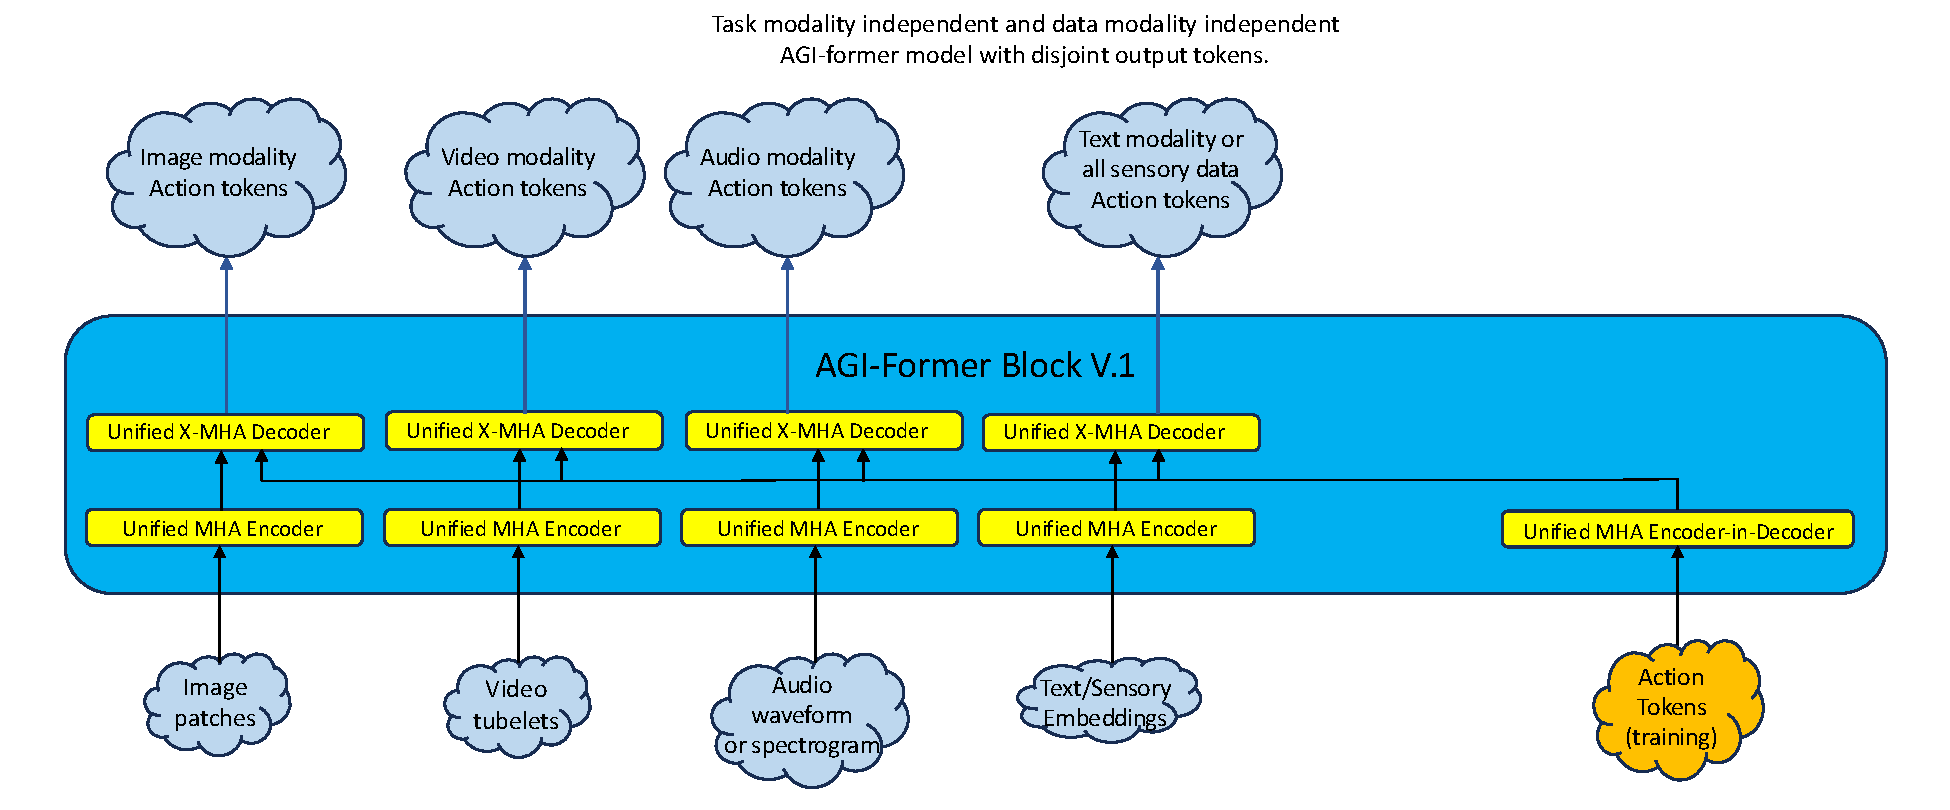
\includegraphics[width=\textwidth]{Figures/fig2.pdf}
    \caption{Disjoint-output AGI-Former. Modality-native inputs are encoded independently, while a shared causal thought--action state conditions one Unified Cross-MHA decoder per modality. Each branch retains a separate output-token space. Ground-truth history is supplied during teacher-forced training; generated history is used autoregressively during inference.}
    \label{fig:agi_former_disjoint}
\end{figure*}

\subsection{\textbf{Unified Modality Encoders}}

Let $\mathcal{M}_{\mathrm{out}}\subseteq\mathcal{M}$ denote the modalities associated with disjoint output branches. Following the notation of Section~III, the token sequence $X_t^{(m)}$ is projected into the common model dimension and encoded as

\begin{equation}
\begin{aligned}
    H_t^{(m)}
    &= \operatorname{UMHAEnc}_{m}\!\left(
       X_t^{(m)};\theta_{E_m}
       \right)
     \in\mathbb{R}^{N_{m,t}\times d},
    &&m\in\mathcal{M}_{\mathrm{out}}.
\end{aligned}
\label{eq:disjoint_modality_encoder}
\end{equation}

Here, $\operatorname{UMHAEnc}_{m}$ denotes a stack of modality-specific Unified MHA encoder blocks derived from the unified-attention formulation of UTR \cite{zohourian2026utr}. The encoders need not share parameters or sequence lengths. Their common output width $d$ defines the interface through which the action state can attend to any branch.

For a missing modality, no synthetic observation is required. Let $r_t^{(m)}\in\{0,1\}$ indicate whether modality $m$ is available at step $t$. The active encoded set is

\begin{equation}
\begin{aligned}
    \mathcal{H}_t
    &= \left\{
       H_t^{(m)}:
       m\in\mathcal{M}_{\mathrm{out}},\;
       r_t^{(m)}=1
       \right\}.
\end{aligned}
\label{eq:active_modalities}
\end{equation}

This definition permits asynchronous sensors and modality dropout without changing the parameterization of the remaining branches.

\subsection{\textbf{Shared Causal Thought--Action State}}

The architecture uses one causal state to condition all disjoint branches. During teacher-forced training, let $\widetilde{Y}_{<t}$ denote the ground-truth thought--action history shifted by one token. During inference, let $\widehat{Y}_{<t}$ contain the tokens generated by the model. The history supplied to the encoder-in-decoder is therefore

\begin{equation}
\begin{aligned}
    Y^{\star}_{<t}
    &=
    \begin{cases}
        \widetilde{Y}_{<t}, & \text{training},\\
        \widehat{Y}_{<t},   & \text{inference},
    \end{cases}\\
    S_t
    &= \operatorname{UMHAED}\!\left(
       Y^{\star}_{<t};\theta_{A}
       \right)
     \in\mathbb{R}^{L_{<t}\times d},
\end{aligned}
\label{eq:disjoint_action_state}
\end{equation}

where $\operatorname{UMHAED}$ is the masked Unified MHA encoder-in-decoder shown in Fig.~\ref{fig:agi_former_disjoint}. The causal mask prevents a position from accessing future thought or action tokens.

Because the branches generate different streams, their completed outputs must be represented consistently in the next decision history. Let $\rho$ be a deterministic serialization operator that inserts branch identifiers, temporal markers, and termination tokens before interleaving or concatenating the outputs:

\begin{equation}
\begin{aligned}
    Y_t
    &= \rho\!\left(
       \left\{y_t^{(m)}\right\}_{m\in\mathcal{M}_{\mathrm{out}}}
       \right),\\
    Y_{<t+1}
    &= \left[Y_{<t};Y_t\right].
\end{aligned}
\label{eq:disjoint_history_update}
\end{equation}

The operator $\rho$ does not fuse branch representations. It only records what each branch produced so that later decisions can be conditioned on the complete prior behavior of the agent.

\subsection{\textbf{Per-Modality Unified Cross-Attention}}

For each available modality, a Unified X-MHA decoder uses the causal state as the decoding stream and the modality encoding as its conditioning stream. We denote the branch output by

\begin{equation}
\begin{aligned}
    Z_t^{(m)}
    &= \operatorname{UXMHADec}_{m}\!\left(
       S_t,H_t^{(m)};\theta_{D_m}
       \right)
     \in\mathbb{R}^{L_t^{(m)}\times d},\\
    &\hspace{7.2cm}
       m\in\mathcal{M}_{\mathrm{out}},\;r_t^{(m)}=1.
\end{aligned}
\label{eq:disjoint_cross_attention}
\end{equation}

The ordering of the arguments is significant: $S_t$ determines the current decision context, and $H_t^{(m)}$ supplies the modality-native evidence relevant to that context. The Unified X-MHA operation is independently parameterized for each branch unless parameter sharing is imposed as an experimental constraint. This independence allows image, video, audio, language, and actuator branches to learn different attention patterns while receiving the same causal history.

Residual and feedforward processing at branch $m$ and layer $\ell$ can be written as

\begin{equation}
\begin{aligned}
    C_{t,\ell}^{(m)}
    &= \operatorname{LN}\!\left(
       S_{t,\ell}^{(m)}+
       \operatorname{UXMHA}_{m,\ell}\!\left(
       S_{t,\ell}^{(m)},H_t^{(m)}
       \right)
       \right),\\
    S_{t,\ell+1}^{(m)}
    &= \operatorname{LN}\!\left(
       C_{t,\ell}^{(m)}+
       \operatorname{FFN}_{m,\ell}\!\left(C_{t,\ell}^{(m)}\right)
       \right).
\end{aligned}
\label{eq:disjoint_decoder_layer}
\end{equation}

Equation~\eqref{eq:disjoint_decoder_layer} specifies the branch interface without constraining the internal unified-attention parameterization, which follows UTR and can be varied through ablation.

\subsection{\textbf{Independent Output Heads and Training Objective}}

Each branch maps its decoder representation to its own output space $\mathcal{V}_m$. For discrete action tokens,

\begin{equation}
\begin{aligned}
    P_t^{(m)}
    &= \operatorname{softmax}\!\left(
       Z_t^{(m)}W_{O}^{(m)}+b_{O}^{(m)}
       \right),\\
    \widehat{y}_{t,j}^{(m)}
    &\sim P_t^{(m)}[j,:],
    &&j=1,\ldots,L_t^{(m)}.
\end{aligned}
\label{eq:disjoint_output_head}
\end{equation}

Continuous actions may instead be represented by quantized tokens or predicted through a distributional regression head. Keeping $W_O^{(m)}$ branch specific avoids requiring semantically unrelated outputs to share a vocabulary.

Let $q_t^{(m)}\in\{0,1\}$ indicate that a target output is available for branch $m$ at step $t$. The multi-branch training objective is

\begin{equation}
\begin{aligned}
    \mathcal{L}_{\mathrm{dis}}
    &= \sum_{m\in\mathcal{M}_{\mathrm{out}}}
       \lambda_m
       \sum_{t=1}^{T}q_t^{(m)}
       \mathcal{L}_{m,t},\\
    \mathcal{L}_{m,t}
    &= -\sum_{j=1}^{L_t^{(m)}}
       \log P_t^{(m)}
       \!\left[j,y_{t,j}^{(m)}\right],\\
    \lambda_m&\geq0,
    \qquad
    \sum_{m\in\mathcal{M}_{\mathrm{out}}}\lambda_m=1.
\end{aligned}
\label{eq:disjoint_loss}
\end{equation}

The weights $\lambda_m$ prevent branches with longer sequences or denser supervision from dominating optimization. They may be fixed, uncertainty weighted, or adapted according to gradient balance. When the encoders and causal-state module are trainable, gradients from every supervised branch update the shared perception--state--action system, while each output head retains its own semantics.

\subsection{\textbf{Inference and Branch Coordination}}

At inference, all active branches can decode in parallel after $S_t$ and their respective $H_t^{(m)}$ have been computed. A branch terminates when it produces its end token or satisfies an actuator-specific stopping rule. If simultaneous outputs are permitted, the environment executes the resulting set. If outputs compete for one resource, a deterministic safety or scheduling policy $\Pi$ selects an executable subset:

\begin{equation}
\begin{aligned}
    \widehat{\mathcal{Y}}_t^{\mathrm{dis}}
    &= \left\{
       \widehat{y}_t^{(m)}:
       m\in\mathcal{M}_{\mathrm{out}},\;r_t^{(m)}=1
       \right\},\\
    \mathcal{E}_t
    &= \Pi\!\left(
       \widehat{\mathcal{Y}}_t^{\mathrm{dis}},c_t
       \right),
\end{aligned}
\label{eq:disjoint_execution}
\end{equation}

where $c_t$ contains environmental constraints, permissions, and safety rules. The policy $\Pi$ is not a substitute for learned joint reasoning; it prevents incompatible commands from being executed when the architecture intentionally retains disjoint outputs.

\subsection{\textbf{Capabilities and Limitations}}

The disjoint architecture provides four practical advantages. First, it accommodates heterogeneous output spaces without a universal action vocabulary. Second, branches can be trained with partially labeled datasets because $q_t^{(m)}$ masks unavailable targets. Third, branch-specific representations and heads make modality-level errors easier to isolate. Fourth, independent branches can be added or replaced without retraining every output projection, although changes to shared components may still require joint adaptation.

Its central limitation is the absence of a final learned fusion stage. Branches share prior history but do not directly negotiate their current outputs before generation. Conflicts may therefore be resolved only at the next autoregressive step or by the execution policy $\Pi$. Computation also grows with the number and length of active branches, and independently optimized losses can generate negative transfer through shared components. These limitations motivate the joint-output architecture in Section~V, where action-conditioned modality representations are combined before the final action sequence is generated.

\section{\textbf{Joint-Output AGI-Former}}

The joint-output architecture extends AGI-Former from parallel outputs conditioned separately by each modality to one coordinated thought--action sequence. Its defining operation is not concatenation alone, but the placement of concatenation after each modality has been conditioned on the current causal state. Each branch first selects and transforms the evidence relevant to the pending decision. The selected representations are then assembled into a multimodal memory that conditions a final Unified Cross-MHA decoder.

Figure~\ref{fig:agi_former_joint} presents this organization. The modality encoders and causal Unified MHA encoder-in-decoder retain the roles defined in Sections~III and IV. Unlike the disjoint architecture, however, the outputs of the first-stage Unified X-MHA decoders are intermediate action-conditioned representations rather than independently executable commands. Concatenation combines these representations, and a second Unified X-MHA decoder generates the joint output tokens.

\begin{figure*}[t]
    \centering
    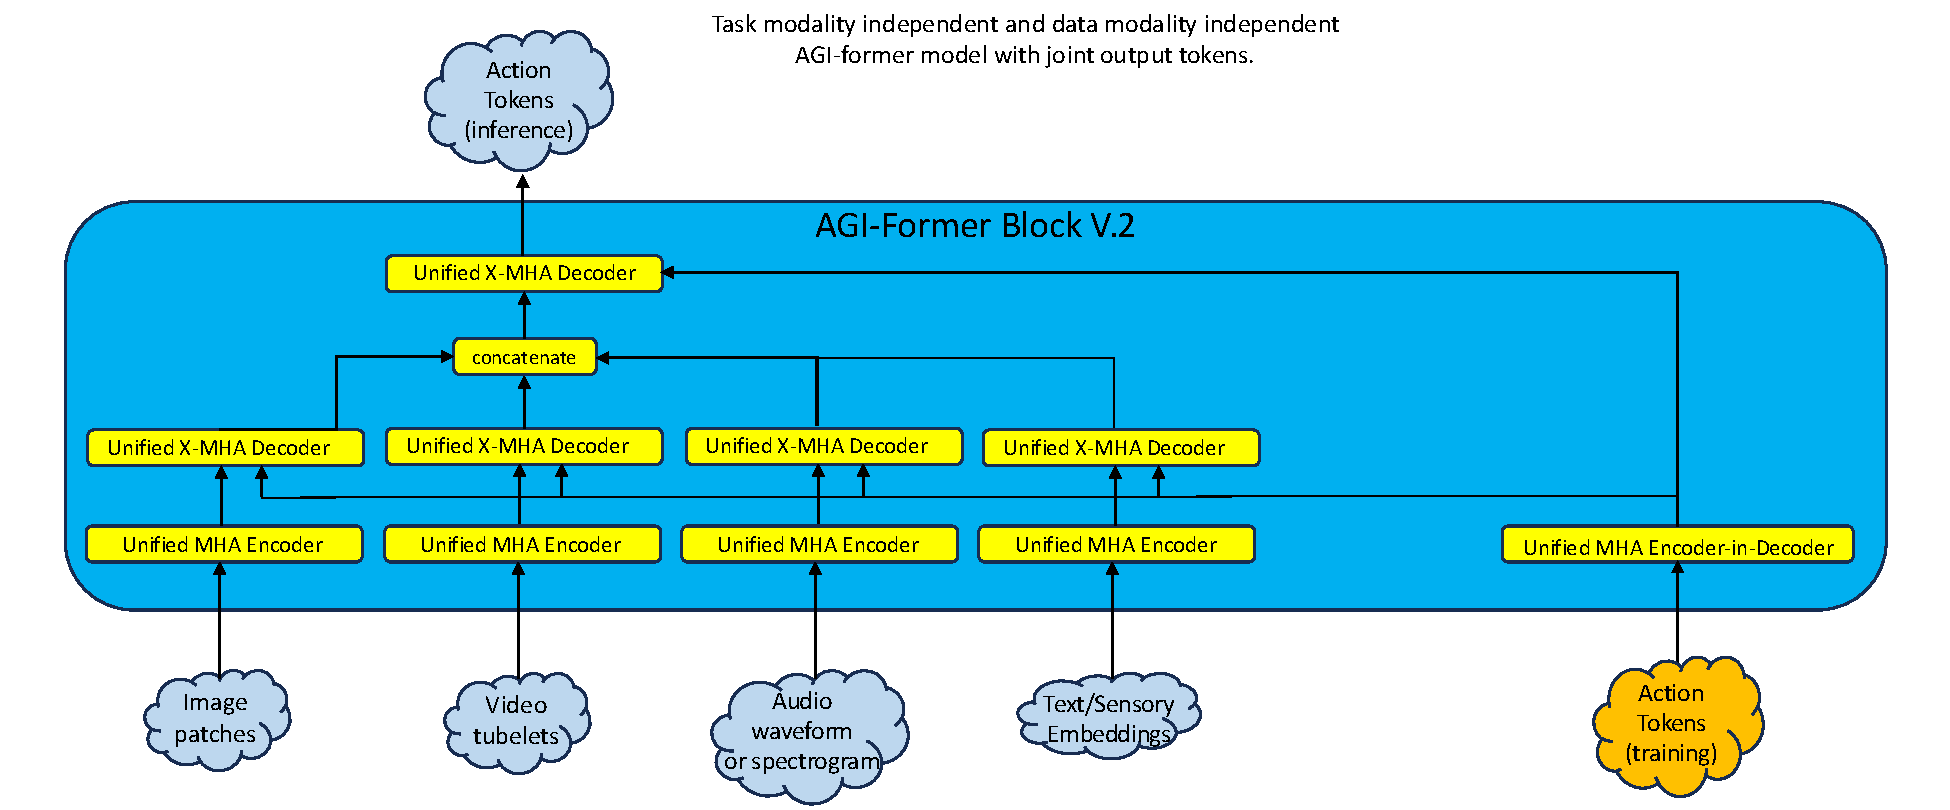
\includegraphics[width=\textwidth]{Figures/fig3.pdf}
    \caption{Joint-output AGI-Former. Each modality is encoded independently and conditioned on the shared causal thought--action state through a first-stage Unified Cross-MHA decoder. The conditioned representations are concatenated into a multimodal memory. A final Unified Cross-MHA decoder attends to that memory from the same causal state and generates one coordinated action-token sequence.}
    \label{fig:agi_former_joint}
\end{figure*}

\subsection{\textbf{First-Stage Action-Conditioned Representations}}

For each available modality $m\in\mathcal{M}$, the Unified MHA encoder produces $H_t^{(m)}$ as defined in Eq.~\eqref{eq:disjoint_modality_encoder}. The causal Unified MHA encoder-in-decoder produces $S_t$ from ground-truth history during training or generated history during inference according to Eq.~\eqref{eq:disjoint_action_state}. A first-stage Unified X-MHA decoder then computes

\begin{equation}
\begin{aligned}
    R_t^{(m)}
    &= \operatorname{UXMHA}^{(1)}_{m}\!\left(
       S_t,H_t^{(m)};\theta_{C_m}
       \right)
     \in\mathbb{R}^{L_t\times d},\\
    &\hspace{7.2cm}
       m\in\mathcal{M},\;r_t^{(m)}=1.
\end{aligned}
\label{eq:joint_conditioned_modality}
\end{equation}

The shared query length $L_t$ aligns every $R_t^{(m)}$ with the current thought--action state while permitting the encoded memories $H_t^{(m)}$ to retain different lengths. Thus, an image branch may attend over spatial patches, a video branch over tubelets, an audio branch over temporal or spectrogram tokens, and a language branch over text or sensor embeddings without requiring equal input geometry.

The intermediate representation $R_t^{(m)}$ is not interpreted as a complete action from modality $m$. It represents the evidence selected from that modality in response to the current causal state. This distinction separates joint AGI-Former from a voting or post-hoc aggregation system: the branches produce decision-conditioned evidence, not competing final decisions.

\subsection{\textbf{Action-Conditioned Late Fusion}}

Let $e_m\in\mathbb{R}^{d}$ be a learned modality-identity embedding broadcast across the positions of branch $m$. The active branch representations are concatenated along the token axis:

\begin{equation}
\begin{aligned}
    F_t
    &= \mathop{\operatorname{Concat}}_{m\in\mathcal{M}:r_t^{(m)}=1}
       \left(R_t^{(m)}+\mathbf{1}_{L_t}e_m^{\top}\right),\\
    F_t
    &\in\mathbb{R}^{L_t|\mathcal{M}_t|\times d},\\
    \mathcal{M}_t
    &= \left\{m\in\mathcal{M}:r_t^{(m)}=1\right\}.
\end{aligned}
\label{eq:joint_concatenation}
\end{equation}

The modality embeddings preserve source identity after concatenation. Positional or temporal embeddings remain attached to the tokens within each branch. A fusion mask $B_t$ identifies valid positions when branch sequences are padded or batched:

\begin{equation}
\begin{aligned}
    B_t[i]
    &=
    \begin{cases}
        0,       & \text{if }F_t[i,:]\text{ is valid},\\
        -\infty, & \text{if }F_t[i,:]\text{ is padding}.
    \end{cases}
\end{aligned}
\label{eq:joint_fusion_mask}
\end{equation}

Because each $R_t^{(m)}$ is already conditioned on $S_t$, Eq.~\eqref{eq:joint_concatenation} implements action-conditioned late fusion. An early-fusion alternative would concatenate $H_t^{(m)}$ before any branch-specific interaction with the causal state. That alternative is a valid ablation, but it asks a single fusion stage to discover both within-modality relevance and cross-modal coordination simultaneously.

\subsection{\textbf{Final Unified Cross-MHA Synthesis}}

The final Unified X-MHA decoder uses the causal state as its decoding stream and the concatenated representation $F_t$ as multimodal memory:

\begin{equation}
\begin{aligned}
    J_t
    &= \operatorname{UXMHA}^{(2)}\!\left(
       S_t,F_t,B_t;\theta_J
       \right)
     \in\mathbb{R}^{L_t\times d}.
\end{aligned}
\label{eq:joint_final_decoder}
\end{equation}

At final decoder layer $\ell$, the corresponding residual computation is

\begin{equation}
\begin{aligned}
    U_{t,\ell}
    &= \operatorname{LN}\!\left(
       J_{t,\ell}+
       \operatorname{UXMHA}^{(2)}_{\ell}\!\left(
       J_{t,\ell},F_t,B_t
       \right)
       \right),\\
    J_{t,\ell+1}
    &= \operatorname{LN}\!\left(
       U_{t,\ell}+
       \operatorname{FFN}^{(2)}_{\ell}\!\left(U_{t,\ell}\right)
       \right).
\end{aligned}
\label{eq:joint_final_layer}
\end{equation}

This second attention stage can compare evidence selected independently from different modalities. It may, for example, align an observed object with a spoken instruction, reconcile motion in video with a sound event, or suppress a text hypothesis contradicted by current sensory evidence. The output remains conditioned on $S_t$, preserving continuity with prior decisions rather than treating the fused memory as an isolated multimodal sample.

\subsection{\textbf{Joint Output Space}}

Let $\mathcal{V}_{J}$ be the vocabulary of the joint output stream. It may include natural-language tokens, internal control tokens, tool identifiers, action-type markers, quantized control values, and termination symbols. The next-token distribution is

\begin{equation}
\begin{aligned}
    P_t^{J}
    &= \operatorname{softmax}\!\left(
       J_tW_O^{J}+b_O^{J}
       \right),\\
    \widehat{y}_{t,j}^{J}
    &\sim P_t^{J}[j,:],
    &&j=1,\ldots,L_t.
\end{aligned}
\label{eq:joint_output_head}
\end{equation}

An output grammar or typed-token mask $G_{t,j}\in\{0,-\infty\}^{|\mathcal{V}_J|}$ can prohibit syntactically or physically invalid tokens:

\begin{equation}
\begin{aligned}
    P_{t,j}^{J}
    &= \operatorname{softmax}\!\left(
       z_{t,j}^{J}W_O^{J}+b_O^{J}+G_{t,j}
       \right).
\end{aligned}
\label{eq:joint_typed_mask}
\end{equation}

The mask constrains output validity but does not determine which valid action should be selected. That decision remains learned from the joint representation.

\subsection{\textbf{Training Objective}}

For teacher-forced training, the principal joint loss is the negative log-likelihood of the target output sequence:

\begin{equation}
\begin{aligned}
    \mathcal{L}_{J}
    &= -\sum_{t=1}^{T}
       \sum_{j=1}^{L_t}
       \log P_{t,j}^{J}\!\left[y_{t,j}^{J}\right].
\end{aligned}
\label{eq:joint_primary_loss}
\end{equation}

A model trained only through $\mathcal{L}_{J}$ could underuse one or more branches when another modality predicts the target sufficiently well. Optional auxiliary losses can preserve branch-level grounding:

\begin{equation}
\begin{aligned}
    \mathcal{L}_{\mathrm{joint}}
    &= \mathcal{L}_{J}
       +\sum_{m\in\mathcal{M}}
        \alpha_m\mathcal{L}_{\mathrm{aux}}^{(m)}
       +\beta\mathcal{L}_{\mathrm{align}}
       +\gamma\mathcal{L}_{\mathrm{reg}},\\
    \alpha_m,\beta,\gamma&\geq0.
\end{aligned}
\label{eq:joint_total_loss}
\end{equation}

Here, $\mathcal{L}_{\mathrm{aux}}^{(m)}$ may predict branch-relevant targets, $\mathcal{L}_{\mathrm{align}}$ may encourage correspondence across synchronized modalities, and $\mathcal{L}_{\mathrm{reg}}$ may include modality-dropout or attention-entropy regularization. These terms are optional and must be ablated; the defining joint architecture is given by Eqs.~\eqref{eq:joint_conditioned_modality}--\eqref{eq:joint_final_decoder}.

During training, modality dropout samples subsets $\mathcal{M}_t\subseteq\mathcal{M}$ so that the final decoder cannot assume that every stream is always present. For a retention probability $p_m$,

\begin{equation}
\begin{aligned}
    r_t^{(m)}&\sim\operatorname{Bernoulli}(p_m),\\
    \mathcal{M}_t&=\left\{m:r_t^{(m)}=1\right\},
    \qquad
    |\mathcal{M}_t|\geq1.
\end{aligned}
\label{eq:joint_modality_dropout}
\end{equation}

This procedure trains one parameterization over variable modality sets and supports direct testing of robustness to missing or corrupted inputs.

\subsection{\textbf{Autoregressive Inference}}

At inference step $j$, the model recomputes or caches the causal state, conditions each available modality, constructs $F_t$, and samples or selects the next joint token. The recurrence is

\begin{equation}
\begin{aligned}
    S_{t,j}
    &= \operatorname{UMHAED}\!\left(
       \widehat{Y}_{<t},\widehat{y}_{t,<j}^{J}
       \right),\\
    R_{t,j}^{(m)}
    &= \operatorname{UXMHA}^{(1)}_m\!\left(
       S_{t,j},H_t^{(m)}
       \right),\\
    F_{t,j}
    &= \operatorname{Concat}_{m\in\mathcal{M}_t}
       \left(R_{t,j}^{(m)}+e_m\right),\\
    \widehat{y}_{t,j}^{J}
    &\sim p_{\theta}\!\left(
       \cdot\mid S_{t,j},F_{t,j}
       \right).
\end{aligned}
\label{eq:joint_inference}
\end{equation}

Caching encoder outputs and past decoder states avoids repeating computations that do not change within the decision step. When new sensor measurements arrive during generation, only the affected branch and downstream fusion computations need to be refreshed.

\subsection{\textbf{Complexity and Architectural Tradeoffs}}

Let $L$ denote the causal-state length and $N_m$ the encoded length of modality $m$. Ignoring encoder-internal costs and constants associated with attention heads, first-stage cross-attention requires

\begin{equation}
\begin{aligned}
    \mathcal{C}_{1}
    &= \mathcal{O}\!\left(
       dL\sum_{m\in\mathcal{M}_t}N_m
       \right).
\end{aligned}
\label{eq:joint_stage_one_complexity}
\end{equation}

Concatenation produces $L|\mathcal{M}_t|$ memory tokens. The final cross attention therefore requires

\begin{equation}
\begin{aligned}
    \mathcal{C}_{2}
    &= \mathcal{O}\!\left(
       dL^2|\mathcal{M}_t|
       \right).
\end{aligned}
\label{eq:joint_stage_two_complexity}
\end{equation}

The second stage is the principal additional cost relative to disjoint branches. Token pooling, learned compression, sparse attention, or branch selection may reduce this cost, but each changes the information available for joint synthesis and must therefore be evaluated rather than assumed equivalent.

The joint architecture resolves the principal limitation of the disjoint design: all active modalities influence one learned output before execution. It also introduces new risks. A dominant modality may suppress weaker streams; concatenation increases memory; conflicting evidence may destabilize attention; and one shared output vocabulary can become difficult to balance across heterogeneous action types. The disjoint and joint models should therefore be treated as alternative hypotheses whose relative value depends on the task, output semantics, training data, and deployment constraints. Section~VI develops the experimental protocol needed to compare them.

\section{\textbf{Hierarchical Joint--Disjoint Agency}}

The disjoint and joint AGI-Former architectures need not be deployed as mutually exclusive alternatives. They can be composed into a hierarchy in which the joint-output architecture performs global coordination and disjoint-output architectures perform regional or specialized execution. In this organization, the global model generates unified supervisory action tokens that express a shared plan, while each regional model translates that plan into actions valid for its local observations, capabilities, and constraints.

Figure~\ref{fig:hierarchical_agi_former} illustrates the resulting recurrent control loop. Regional agents receive local multimodal observations and return state representations, action proposals, uncertainty estimates, and execution feedback. The global joint coordinator fuses this information and produces supervisory tokens encoding goals, priorities, constraints, or a coordinated plan. Those tokens condition the regional agents, which produce locally executable actions. Environmental consequences then generate new observations and feedback for the next cycle.

\begin{figure*}[t]
    \centering
    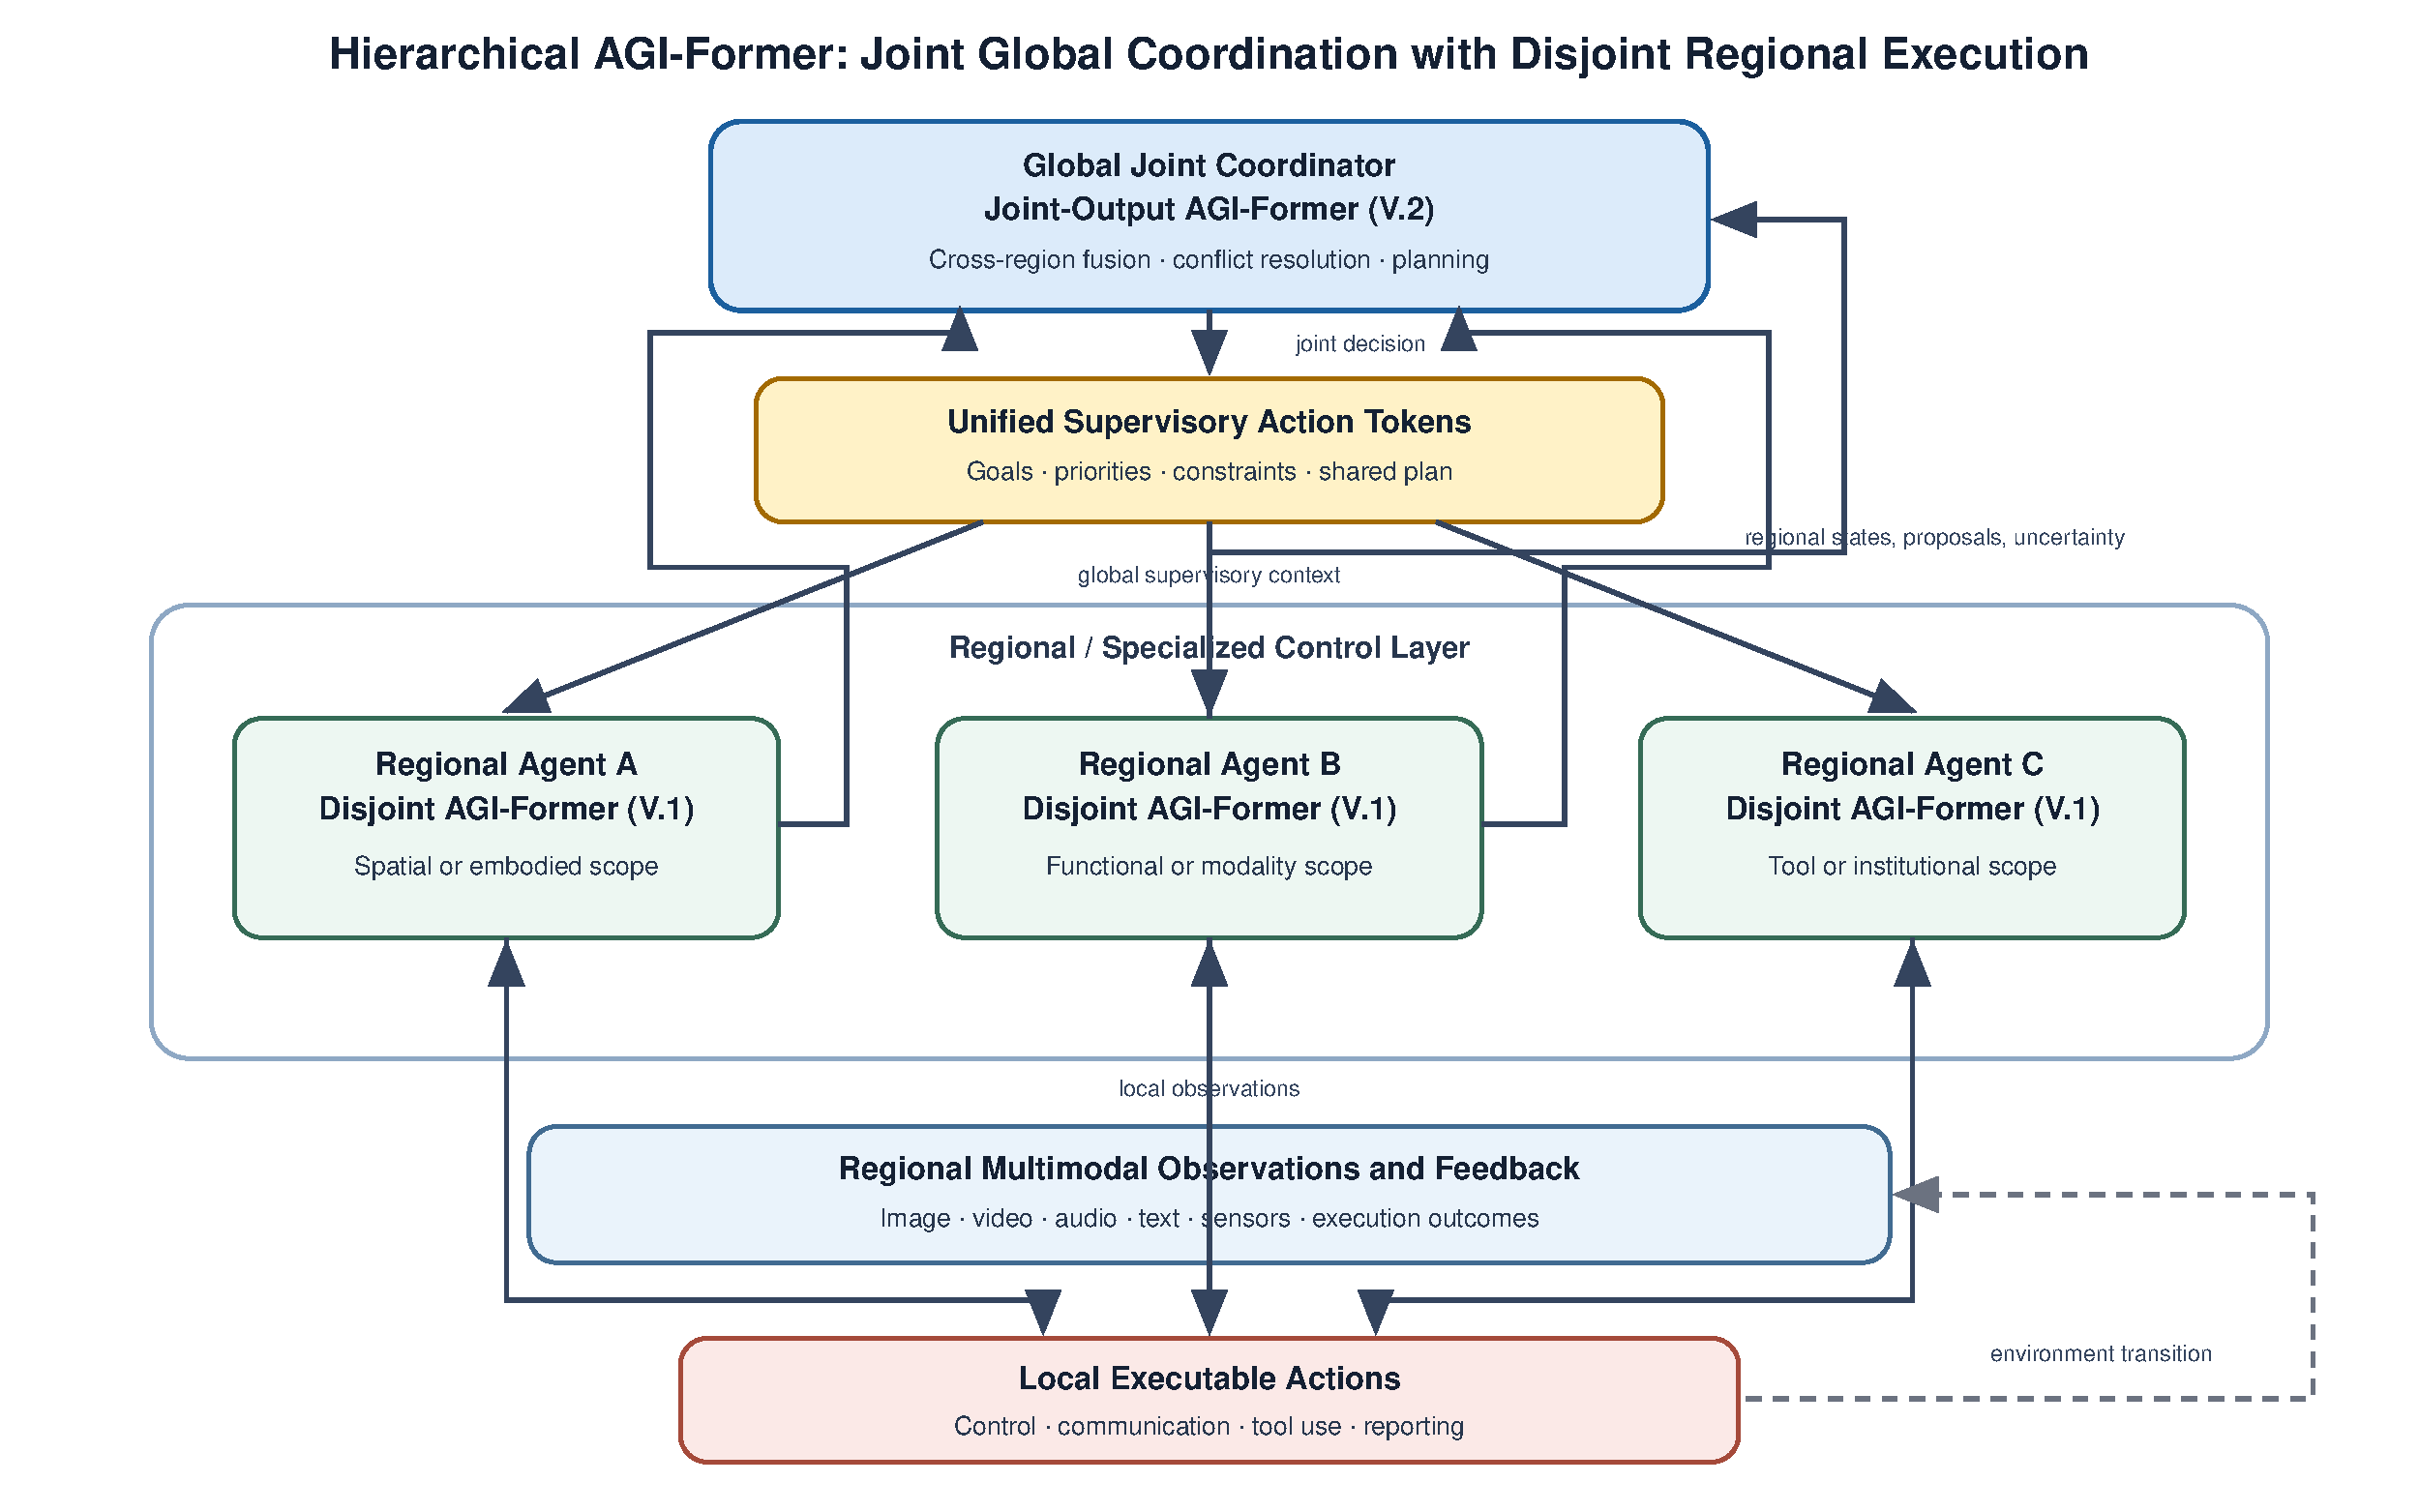
\includegraphics[width=\textwidth]{Figures/fig4.pdf}
    \caption{Hierarchical AGI-Former with joint global coordination and disjoint regional execution. Regional AGI-Former agents transform local observations and global supervisory context into specialized actions. Their states, proposals, uncertainty, and execution feedback are aggregated by a joint-output AGI-Former, which generates the supervisory tokens for the next control cycle.}
    \label{fig:hierarchical_agi_former}
\end{figure*}

\subsection{\textbf{Regional Agents and Scope}}

Let $\mathcal{R}=\{1,\ldots,R\}$ denote a set of regional agents. A region need not be geographic. It may correspond to a physical zone, robot, actuator group, modality, functional capability, software tool, institution, or administrative jurisdiction. Agent $r$ receives a local modality set $\mathcal{M}_r$ and maintains a local causal history $Y_{<t}^{(r)}$. Its encoded local context is

\begin{equation}
\begin{aligned}
    \mathcal{H}_t^{(r)}
    &= \left\{
       E_m^{(r)}\!\left(X_t^{(r,m)}\right):
       m\in\mathcal{M}_r,\;r_t^{(r,m)}=1
       \right\},\\
    S_t^{(r)}
    &= \operatorname{UMHAED}^{(r)}\!\left(
       Y_{<t}^{(r)}
       \right).
\end{aligned}
\label{eq:regional_context}
\end{equation}

Each regional agent is therefore an instance of the disjoint architecture, but its branches and output spaces may differ from those of other regions. A drone region may produce navigation and camera-control tokens, while a communication region may produce language and network-action tokens.

Let $s_r$ be a learned or structured scope token identifying the authority and capabilities of region $r$. Scope is included in both upward and downward communication so that identical token values cannot silently acquire different operational meanings across agents.

\subsection{\textbf{Upward Regional State and Proposal Tokens}}

Before the global decision, each regional agent compresses its current context into a bounded upward message:

\begin{equation}
\begin{aligned}
    q_t^{(r)}
    &= \operatorname{RegionalReadout}_{r}\!\left(
       S_t^{(r)},\mathcal{H}_t^{(r)},s_r
       \right),\\
    q_t^{(r)}
    &= \left[
       q_{t,\mathrm{state}}^{(r)};
       q_{t,\mathrm{proposal}}^{(r)};
       q_{t,\mathrm{uncertainty}}^{(r)};
       q_{t,\mathrm{feedback}}^{(r)}
       \right].
\end{aligned}
\label{eq:regional_upward_message}
\end{equation}

The four fields are logical token types rather than mandatory fixed-length vectors. State tokens describe locally relevant conditions; proposal tokens express candidate actions or requested resources; uncertainty tokens communicate confidence, missing information, or conflict; and feedback tokens summarize the outcome of previously executed commands.

The active regional messages form the global input memory

\begin{equation}
\begin{aligned}
    Q_t
    &= \mathop{\operatorname{Concat}}_{r\in\mathcal{R}_t}
       \left(q_t^{(r)}+e_r\right),\\
    \mathcal{R}_t
    &= \left\{r\in\mathcal{R}:a_t^{(r)}=1\right\},
\end{aligned}
\label{eq:global_regional_memory}
\end{equation}

where $e_r$ identifies the source region and $a_t^{(r)}$ indicates its availability. Regional dropout during training can vary $\mathcal{R}_t$ so that global coordination does not depend on every agent being continuously reachable.

\subsection{\textbf{Global Joint Coordination}}

The global coordinator is an instance of the joint-output architecture. It conditions its global causal state $S_k^{G}$ on $Q_t$ and generates a unified supervisory sequence $u_k$:

\begin{equation}
\begin{aligned}
    J_k^{G}
    &= \operatorname{JointAGIFormer}\!\left(
       S_k^{G},Q_t;\theta_G
       \right),\\
    u_k
    &\sim p_{\theta_G}\!\left(
       u_k\mid S_k^{G},Q_t
       \right).
\end{aligned}
\label{eq:global_supervision}
\end{equation}

The supervisory sequence may contain a global objective, ordered subgoals, resource assignments, temporal constraints, prohibitions, escalation conditions, and region-addressed directives. It is a learned action-token sequence, not merely a natural-language summary.

To prevent every region from receiving every directive, let $A_k\in\{0,1\}^{R\times |u_k|}$ be an address and authorization mask. The supervisory context visible to region $r$ is

\begin{equation}
\begin{aligned}
    u_k^{(r)}
    &= \operatorname{Select}\!\left(
       u_k,A_k[r,:],s_r
       \right).
\end{aligned}
\label{eq:regional_supervision_mask}
\end{equation}

This mechanism distinguishes shared plan tokens from restricted commands and allows the hierarchy to represent different permissions, capabilities, or information boundaries.

\subsection{\textbf{Regional Execution Under Global Context}}

Each regional agent treats $u_k^{(r)}$ as an additional causal condition rather than as an executable command by itself. The regional action distribution is

\begin{equation}
\begin{aligned}
    y_t^{(r)}
    &\sim p_{\theta_r}\!\left(
       y_t^{(r)}
       \mid S_t^{(r)},
       \mathcal{H}_t^{(r)},
       u_k^{(r)},
       c_t^{(r)}
       \right),
\end{aligned}
\label{eq:regional_execution}
\end{equation}

where $c_t^{(r)}$ contains local physical, legal, resource, and safety constraints. The disjoint regional architecture can emit several specialized streams when a region controls multiple tools or effectors. Thus, one global sequence may generate many locally valid actions without requiring a universal low-level control vocabulary.

The environment transition and feedback loop are

\begin{equation}
\begin{aligned}
    e_{t+1}
    &\sim \mathcal{P}\!\left(
       e_{t+1}\mid e_t,
       \{y_t^{(r)}\}_{r\in\mathcal{R}_t}
       \right),\\
    f_{t+1}^{(r)}
    &= \operatorname{FeedbackEnc}_{r}\!\left(
       x_{t+1}^{(r)},y_t^{(r)},c_{t+1}^{(r)}
       \right),\\
    q_{t+1,\mathrm{feedback}}^{(r)}
    &\leftarrow f_{t+1}^{(r)}.
\end{aligned}
\label{eq:hierarchical_feedback}
\end{equation}

The next global decision therefore depends on observed consequences, not solely on whether regional agents accepted the previous plan.

\subsection{\textbf{Multiple Control Time Scales}}

Global coordination and regional execution need not occur at the same frequency. Let $k$ index global planning intervals and let $t\in[b_k,b_{k+1})$ index local decisions governed by supervisory sequence $u_k$. Then

\begin{equation}
\begin{aligned}
    u(t)&=u_k,
    &&b_k\leq t<b_{k+1},\\
    b_{k+1}
    &=\min\left\{
       t>b_k:
       \operatorname{Replan}(f_{\leq t},u_k)=1
       \right\}.
\end{aligned}
\label{eq:hierarchical_timescale}
\end{equation}

Replanning may be periodic or event triggered by goal completion, unexpected observations, resource conflict, uncertainty, safety violations, or loss of communication. This separation allows fast regional control beneath slower global deliberation.

\subsection{\textbf{Hierarchical Training Objective}}

The hierarchy can be trained in stages or jointly. A staged procedure can first train regional perception and action, then train global coordination over frozen or partially frozen regional interfaces, and finally fine-tune the complete loop. A joint objective can be written as

\begin{equation}
\begin{aligned}
    \mathcal{L}_{H}
    &= \lambda_G\mathcal{L}_{G}
       +\sum_{r\in\mathcal{R}}
        \lambda_r\mathcal{L}_{r}
       +\eta\mathcal{L}_{\mathrm{coord}}
       +\mu\mathcal{L}_{\mathrm{cons}}
       +\nu\mathcal{L}_{\mathrm{safe}},\\
    \lambda_G,\lambda_r,\eta,\mu,\nu&\geq0.
\end{aligned}
\label{eq:hierarchical_loss}
\end{equation}

Here, $\mathcal{L}_{G}$ supervises global plans, $\mathcal{L}_{r}$ supervises regional outputs, $\mathcal{L}_{\mathrm{coord}}$ measures collective task success, $\mathcal{L}_{\mathrm{cons}}$ penalizes contradictions between global directives and regional actions, and $\mathcal{L}_{\mathrm{safe}}$ penalizes invalid or unsafe behavior. Because global success can be delayed and sparsely observed, behavioral cloning, offline trajectories, simulation, reinforcement learning, or combinations of these methods may supply the optimization signals.

\subsection{\textbf{Resilience and Failure Containment}}

A hierarchy introduces coordination benefits but also creates a potential global bottleneck. Regional agents should therefore define a fallback policy for delayed, unavailable, or invalid supervision:

\begin{equation}
\begin{aligned}
    \pi_r^{\mathrm{exec}}
    &=
    \begin{cases}
       \pi_r(\cdot\mid u_k^{(r)}),
       &\operatorname{Valid}(u_k^{(r)})=1,\\
       \pi_r(\cdot\mid u_{k^-}^{(r)}),
       &\operatorname{Fresh}(u_{k^-}^{(r)})=1,\\
       \pi_r^{\mathrm{safe}},
       &\text{otherwise},
    \end{cases}
\end{aligned}
\label{eq:regional_fallback}
\end{equation}

The safe fallback may stop an actuator, preserve a stable local policy, request human intervention, or restrict outputs to a verified subset. Conversely, the global coordinator should treat missing regional messages as uncertainty rather than as evidence that a region is normal.

The hierarchical architecture therefore combines two complementary forms of agency. Joint tokens express global coordination, while disjoint tokens preserve specialized execution. The resulting loop is more than task routing: regional agents contribute learned state and proposals, the global model produces a shared decision, local models ground that decision in their own observations and constraints, and execution feedback changes subsequent global behavior. Section~VII defines how these claims can be evaluated against flat joint models, independent disjoint agents, and externally routed specialist systems.

\section{\textbf{Experimental Protocol and Testability}}

AGI-Former is an architectural proposal rather than a report of completed training runs. Its scientific value therefore depends on whether its claims can be translated into controlled experiments that may support, weaken, or falsify the proposed mechanisms. This section defines such a protocol. The objective is not to select a benchmark whose aggregate score can be labeled AGI; it is to test whether the architecture improves measurable components of integrated multimodal agency under matched conditions.

\subsection{\textbf{Research Questions and Hypotheses}}

The evaluation should address six primary questions.

\textit{H1---Integration:} Does a jointly trained perception--state--action path outperform an externally routed collection of modality specialists when parameter count, training data, tool access, and inference budget are controlled?

\textit{H2---Action-conditioned fusion:} Does conditioning each modality on the causal thought--action state before fusion improve decisions relative to early fusion of unconditioned modality representations?

\textit{H3---Output organization:} Under which output semantics does a joint stream outperform disjoint streams, and when does branch specialization provide superior accuracy, interpretability, latency, or safety?

\textit{H4---Persistent state:} Does retaining prior thought and action tokens improve long-horizon consistency, recovery from error, and adaptation to feedback relative to a stateless multimodal predictor?

\textit{H5---Hierarchical agency:} Does joint global coordination combined with disjoint regional execution reduce cross-agent conflicts and improve collective task success relative to independent regional agents or a flat joint model?

\textit{H6---Unified attention:} Under otherwise matched conditions, do the UTR-derived Unified MHA and Unified Cross-MHA operations improve optimization, transfer, efficiency, or robustness relative to standard multi-head self- and cross-attention \cite{zohourian2026utr}?

The hypotheses are intentionally comparative. Failure to reject a null hypothesis is informative: it may indicate that a simpler architecture provides equivalent capability or that a proposed mechanism matters only under restricted conditions.

\subsection{\textbf{Compared Systems}}

At minimum, the following systems should be implemented or reproduced.

\begin{itemize}
    \item \textit{Routed specialists:} independently trained modality models whose outputs are converted into text or structured messages and coordinated by a language-model supervisor, following the general orchestration pattern exemplified by HuggingGPT \cite{shen2023hugginggpt}.
    \item \textit{Shared sequence policy:} a decoder-centered generalist model that tokenizes observations and actions within one sequence-modeling interface, following the design direction demonstrated by Gato \cite{reed2022generalist}.
    \item \textit{Unified encoder--decoder:} a shared-token encoder--decoder baseline based on the architectural principles of Unified-IO 2 \cite{lu2024unifiedio2}.
    \item \textit{Disjoint AGI-Former:} the architecture defined in Section~IV.
    \item \textit{Joint AGI-Former:} the action-conditioned late-fusion architecture defined in Section~V.
    \item \textit{Hierarchical AGI-Former:} the global joint and regional disjoint composition defined in Section~VI.
\end{itemize}

Direct comparison requires matched experimental envelopes. Let $P_i$, $C_i$, $D_i$, and $B_i$ denote the trainable parameters, training compute, training data, and inference budget of system $i$. A primary comparison is considered matched only when

\begin{equation}
\begin{aligned}
    \frac{|P_i-P_j|}{\max(P_i,P_j)}&\leq\epsilon_P,\\
    \frac{|C_i-C_j|}{\max(C_i,C_j)}&\leq\epsilon_C,\\
    D_i&=D_j,
    \qquad
    B_i=B_j,
\end{aligned}
\label{eq:matched_budget}
\end{equation}

for predefined tolerances $\epsilon_P$ and $\epsilon_C$. Scaling experiments may relax these conditions, but must be reported separately from architecture-controlled comparisons.

\subsection{\textbf{Task Families and Evaluation Splits}}

No single task family is sufficient. Evaluation should progress through five levels.

\textit{Single-modality competence} verifies that architectural integration does not destroy basic image, video, audio, language, or control capability. \textit{Paired-modality grounding} tests relationships such as vision--language, audio--video, instruction--action, and observation--feedback. \textit{Full multimodal coordination} requires several streams to contribute to one decision. \textit{Embodied interaction} evaluates closed-loop behavior in simulation before physical deployment. \textit{Hierarchical multi-agent tasks} require global planning, regional specialization, communication, and recovery from local failure.

Training and evaluation episodes should be partitioned along several independent axes: familiar versus unseen task compositions, familiar versus unseen environments, observed versus unseen modality combinations, known versus novel action sequences, and intact versus perturbed observations. VIMA-style multimodal manipulation tasks and RT-2-style vision-language-action evaluation provide relevant embodied starting points \cite{jiang2023vima,zitkovich2023rt2}, but the hierarchical model additionally requires environments with multiple regions, effectors, or agents.

Let $\mathcal{D}_{\mathrm{ID}}$ be the in-distribution evaluation set and let $\mathcal{D}_{g}$ denote an evaluation set withholding generalization factor $g$. For metric $M$, the generalization gap is

\begin{equation}
\begin{aligned}
    \operatorname{Gap}_{g}(M)
    &= M\!\left(\mathcal{D}_{\mathrm{ID}}\right)
       -M\!\left(\mathcal{D}_{g}\right).
\end{aligned}
\label{eq:generalization_gap}
\end{equation}

The withheld factor $g$ must be specified before training so that post-hoc dataset selection cannot be used to manufacture an apparent generalization result.

\subsection{\textbf{Performance and Coordination Metrics}}

For $N$ evaluation episodes, task success is

\begin{equation}
\begin{aligned}
    \operatorname{Success}
    &= \frac{1}{N}\sum_{n=1}^{N}
       \mathbb{I}\!\left[
       \operatorname{GoalComplete}(n)=1
       \right].
\end{aligned}
\label{eq:task_success}
\end{equation}

Success should be accompanied by action accuracy, cumulative reward where applicable, invalid-action rate, completion time, and intervention count. For joint or hierarchical tasks, a coordination-conflict rate measures incompatible simultaneous actions:

\begin{equation}
\begin{aligned}
    \operatorname{ConflictRate}
    &= \frac{
       \sum_{n,t}
       \mathbb{I}\!\left[
       \operatorname{Conflict}
       \left(\{y_{n,t}^{(r)}\}_{r\in\mathcal{R}}\right)=1
       \right]
       }{
       \sum_{n,t}
       \mathbb{I}\!\left[
       |\mathcal{R}_{n,t}|>1
       \right]
       }.
\end{aligned}
\label{eq:coordination_conflict}
\end{equation}

Hierarchical evaluation should additionally record directive compliance, regional autonomy under communication loss, replan frequency, time to recover from failed agents, and disagreement between global supervisory tokens and executed local actions.

Cross-modal grounding should be measured through intervention rather than attention visualization alone. For an example whose target depends on modality $m$, let $x^{(m,\mathrm{cf})}$ be a controlled counterfactual that changes the relevant evidence while preserving unrelated content. Grounding sensitivity is

\begin{equation}
\begin{aligned}
    G_m
    &= \mathbb{E}\!\left[
       d_Y\!\left(
       f_{\theta}(x),
       f_{\theta}(x^{(m,\mathrm{cf})})
       \right)
       \right],
\end{aligned}
\label{eq:grounding_intervention}
\end{equation}

where $d_Y$ measures a task-appropriate change in the output distribution or executed action. Counterfactual relevance controls are required: changing an irrelevant feature should not produce the same response magnitude.

\subsection{\textbf{Robustness and Missing Information}}

Robustness tests should independently vary modality absence, corruption, delay, contradiction, and adversarially misleading inputs. Let $\delta$ denote perturbation severity and $M_i(\delta)$ the performance of system $i$. A normalized robustness score over severities $\Delta$ is

\begin{equation}
\begin{aligned}
    R_i
    &= \frac{1}{|\Delta|}
       \sum_{\delta\in\Delta}
       \frac{M_i(\delta)}{M_i(0)}.
\end{aligned}
\label{eq:normalized_robustness}
\end{equation}

Missing-modality tests must distinguish graceful degradation from hidden substitution. A system should not receive a text description generated from a withheld image unless that auxiliary model and its cost are explicitly part of every compared system.

For conflicting modalities, evaluation should measure whether the model detects uncertainty, requests clarification, prioritizes the more reliable source, or produces an unsafe confident action. Calibration metrics should therefore accompany accuracy.

\subsection{\textbf{Ablation Matrix}}

The complete architectures should be compared against mechanism-level ablations:

\begin{itemize}
    \item replace Unified MHA and Unified Cross-MHA with standard attention;
    \item remove the persistent causal thought--action state;
    \item concatenate encoder outputs before action conditioning;
    \item remove modality-identity embeddings;
    \item replace modality-specific encoders with one shared encoder;
    \item remove the final joint decoder;
    \item disable modality and regional dropout;
    \item remove auxiliary grounding losses;
    \item remove the global coordinator from the hierarchy;
    \item hold the supervisory plan fixed instead of replanning from feedback.
\end{itemize}

Each ablation should change one mechanism while preserving parameter count as closely as possible. When exact matching is impossible, a width-adjusted control should determine whether an improvement arises from the mechanism or merely from additional capacity.

\subsection{\textbf{Efficiency and Systems Metrics}}

End-to-end integration may reduce routing and representation-conversion overhead while increasing the cost of joint attention. The evaluation must therefore report training FLOPs, inference FLOPs, peak memory, model storage, wall-clock latency, throughput, communication volume, and energy where measurable. A cost-normalized score can supplement, but not replace, the unnormalized task metrics:

\begin{equation}
\begin{aligned}
    \operatorname{Eff}_{i}(M)
    &= \frac{M_i}{
       \alpha F_i+\beta L_i+\gamma E_i
       },
\end{aligned}
\label{eq:cost_normalized_efficiency}
\end{equation}

where $F_i$, $L_i$, and $E_i$ are inference FLOPs, latency, and energy, and the normalization coefficients must be declared before comparison. Because different deployments value these quantities differently, the complete Pareto frontier should also be reported.

\subsection{\textbf{Statistical Reporting and Reproducibility}}

Every trainable condition should use multiple random seeds and identical data splits. For paired episode scores $z_{i,n}$ and $z_{j,n}$, report the mean paired difference

\begin{equation}
\begin{aligned}
    \widehat{\Delta}_{ij}
    &= \frac{1}{N}\sum_{n=1}^{N}
       \left(z_{i,n}-z_{j,n}\right),
\end{aligned}
\label{eq:paired_effect}
\end{equation}

with confidence intervals obtained from a paired bootstrap or an appropriate hierarchical procedure when episodes are nested within seeds or environments. Statistical significance should be accompanied by effect size and uncertainty. Hypotheses, primary metrics, exclusion criteria, stopping rules, and planned comparisons should be fixed before examining final test performance.

Reproducibility requires release of preprocessing code, tokenizer definitions, model configurations, initialization seeds, training schedules, parameter and compute accounting, evaluation environments, and failed or neutral ablations. Comparisons to closed systems should be labeled observational when weights, training data, or routing logic cannot be controlled.

\subsection{\textbf{Interpretation and Falsification Criteria}}

The evidence would support AGI-Former's architectural claims if improvements are reproducible across task families, survive matched-budget controls, and are attributable to the proposed mechanisms through ablation. The claims would be weakened if routed specialists match the end-to-end models at lower cost, early fusion consistently matches action-conditioned fusion, persistent state provides no long-horizon benefit, joint outputs increase conflicts, or hierarchical coordination fails to outperform independent regional agents.

Even comprehensive positive results would establish neither consciousness nor superintelligence, and they would not by themselves prove AGI. They would provide evidence that a particular end-to-end architecture supports measurable components of integrated multimodal agency. Broader claims require sustained transfer to genuinely novel environments, reliable learning from limited experience, safe long-horizon autonomy, and replication beyond the developers' selected tasks.

\section{\textbf{Discussion, Limitations, and Future Work}}

AGI-Former is intended to convert the general objective of integrated multimodal agency into an explicit and testable neural architecture. Its central departure from externally orchestrated multimodal systems is architectural: modality-specific encoders, causal thought--action representations, cross-modal fusion, and output generation are trained as components of one end-to-end system. This does not imply that every component must share the same parameters or operate at the same temporal resolution. Rather, the proposal requires the components to participate in a common learned decision process whose internal representations and outputs can be optimized jointly.

This distinction matters because a collection of capable specialist models does not automatically constitute an integrated agent. Systems such as HuggingGPT demonstrate that a language model can plan tasks and route requests among external models \cite{shen2023hugginggpt}. Such orchestration is useful, but its interfaces, routing rules, representation conversions, and failure-handling logic are partly imposed outside the learned model. AGI-Former instead asks whether multimodal perception and action can be coupled through a persistent causal state and learned end-to-end. The resulting architecture should therefore be judged by the controlled comparisons in Section~VII, not by the presence of multiple modalities alone.

\subsection{\textbf{Interpretation of the Architectural Variants}}

The disjoint, joint, and hierarchical variants address different output structures. The disjoint architecture is appropriate when modalities, tools, effectors, or regions require distinct vocabularies and independently constrained outputs. Its specialization may improve modularity, diagnosis, and failure containment, but separately generated streams may conflict. The joint architecture produces a unified thought--action sequence and can represent dependencies among outputs directly. Its shared sequence may improve global consistency, although it can also create a bottleneck when several actions must occur concurrently or at substantially different rates.

The hierarchical architecture combines these properties. A joint global model can express a common objective, allocation, or plan, while disjoint regional models translate that supervisory state into locally valid actions. The two output forms are therefore complementary rather than successive claims that one is universally superior. Their relative value depends on action semantics, concurrency, communication constraints, and the scale of the environment. This dependence is why Section~VII treats output organization as an empirical hypothesis.

The same caution applies to Unified Attention. The UTR results motivate Unified MHA and Unified Cross-MHA as candidate operations for integrating self- and cross-attentive computation \cite{zohourian2026utr}; however, transferring those operations from image classification and captioning to multimodal agency is an architectural hypothesis. Only matched ablations can determine whether their benefit persists in the proposed setting.

\subsection{\textbf{Primary Limitation: Integrated Training Data}}

The most immediate limitation is the lack of a coherent training dataset for the complete AGI-Former objective. Existing multimodal datasets usually supervise bounded relationships: an image and caption, a video and description, an audio--visual event, an instruction and robot trajectory, or a question and answer. Multimodal learning research has long identified representation, alignment, translation, fusion, and co-learning as distinct technical challenges \cite{baltrusaitis2019multimodal}. AGI-Former requires these relationships to coexist across time within episodes containing synchronized sensory streams, latent or observable state transitions, thought or planning traces where available, executable actions, environmental consequences, uncertainty, and corrective feedback.

No claim is made here that currently available datasets jointly provide all of these signals at sufficient diversity and scale. Embodied datasets and environments associated with VIMA, PaLM-E, and RT-2 provide useful starting points for multimodal prompting, embodied representation, and vision--language--action learning \cite{jiang2023vima,driess2023palme,zitkovich2023rt2}. Nevertheless, they do not by themselves resolve the broader data requirements of an architecture spanning language, images, audio, video, persistent reasoning, heterogeneous actions, and hierarchical multi-agent feedback.

One possible mitigation is to use videos with rich scientific, technical, or procedural content as surrogate multimodal episodes. A high-quality scientific video may jointly contain temporally ordered visual evidence, speech, text, demonstrations, causal explanations, and observable state changes. Transcripts, diagrams, temporal segments, and demonstrated procedures could be transformed into aligned training targets. Synthetic questions, predictions, action descriptions, and counterfactuals could further enrich an episode.

However, video is not an automatic replacement for interaction data. Passive recordings often omit the decision alternatives considered by an actor, the unobserved state of the environment, the exact action interface, negative outcomes, uncertainty, and feedback following counterfactual choices. Automatically generated annotations may also reproduce errors from the models that generate them. Scientific video should therefore be treated as a promising source for pretraining and dataset construction, not as an established solution. Determining which video domains, annotation procedures, and quality controls produce transferable agency is left to future work.

\subsection{\textbf{Training Cost and Scalability}}

The second major limitation is computational cost. Multiple high-capacity encoders, persistent causal decoding, repeated cross-modal attention, and long action histories may make full end-to-end training substantially more expensive than training or adapting a single-modality model. Video and audio increase sequence length, while the hierarchical architecture adds communication and coordination overhead. Parameter count alone therefore understates the relevant cost; memory, training FLOPs, data preprocessing, communication, inference latency, and energy must also be measured.

Future work will investigate cost reduction rather than assuming that the largest implementation is necessary. Candidate strategies include initializing encoders from pretrained modality models, freezing and progressively unfreezing components, parameter-efficient adaptation, distillation, temporal and spatial token compression, sparse or gated modality activation, cached representations, curriculum learning, and staged training of regional and global models. Perceiver IO and Gato illustrate complementary approaches to structured multimodal input--output processing and generalist sequence modeling \cite{jaegle2022perceiver,reed2022generalist}; AGI-Former experiments should determine which efficiencies can be adopted without removing the proposed action-conditioned integration.

Initial experiments should therefore be deliberately bounded. A small number of modalities, restricted token budgets, compact encoders, and controlled simulated environments can test the architectural mechanisms before expensive scaling. Positive evidence at small scale would not establish that the architecture scales, but negative or neutral ablations could prevent unnecessary large-scale training. Subsequent experiments can increase model capacity, episode length, modality diversity, and the number of regional agents while reporting the matched budgets and Pareto comparisons defined in Section~VII.

\subsection{\textbf{Additional Limitations}}

Several further limitations remain. First, modalities may differ greatly in information density, noise, sampling rate, and dataset size; without careful normalization and sampling, a dominant modality may suppress weaker streams. Second, joint optimization can produce catastrophic interference, in which improvement on one task or modality degrades another. Third, persistent thought--action histories can accumulate errors over long horizons and may consume increasing context without reliable state compression. Fourth, generated action tokens are useful only when grounded in valid action spaces and verified against physical, software, legal, or safety constraints.

Fifth, hierarchical control introduces new failure modes: inaccurate global plans may propagate to several regions, regional messages may be stale or deceptive, and communication loss may divide the system's state. The fallback policies described in Section~VI reduce but do not eliminate these risks. Finally, interpretability remains limited. Attention weights or readable language tokens should not be treated as complete explanations of a decision; causal interventions, execution traces, and controlled counterfactuals are needed to evaluate what information affected an action.

These limitations also define the future-work program. The next steps are to construct coherent multimodal episodes from existing embodied resources and carefully selected scientific videos; define aligned sensory, state, thought, action, and feedback schemas; implement compact disjoint and joint prototypes; perform the mechanism-level ablations in Section~VII; and scale only those components supported by controlled evidence. Later work can examine hierarchical multi-agent deployment, continual adaptation, missing-modality robustness, uncertainty-aware supervision, and safe human intervention.

AGI-Former consequently remains a proposed architecture and research program, not a demonstration of AGI. Even successful experiments would establish evidence for integrated multimodal agency under specified conditions, rather than universal intelligence, consciousness, or superintelligence. This boundary is consistent with the distinction between consciousness and AGI and with the characterization of AGI as integrated multimodal agency developed in prior work \cite{zohourian2026agi}. The contribution of the present paper is to make that characterization implementable, comparable, and falsifiable.

\section{\textbf{Conclusion}}

This paper introduced AGI-Former, a novel and testable end-to-end deep learning architecture for artificial general intelligence. The proposal operationalizes AGI as integrated multimodal agency: the capacity to transform heterogeneous sensory and linguistic information into coherent thought and action across tasks, environments, and time \cite{zohourian2026agi}. Rather than coordinating a discrete collection of specialist models through externally defined routing, AGI-Former places modality-specific encoding, causal thought--action modeling, cross-modal integration, and action generation within a common trainable architecture.

Three complementary organizations were developed. The disjoint architecture generates specialized outputs for modalities, tools, effectors, or regions whose action spaces must remain distinct. The joint architecture produces a unified thought--action sequence after action-conditioned multimodal fusion, allowing dependencies among outputs to be represented directly. The hierarchical architecture combines these forms: a joint global coordinator generates supervisory tokens, while disjoint regional agents ground those tokens in local observations, capabilities, constraints, and feedback. Together, these variants define a progression from integrated perception and action to coordinated multi-agent agency without assuming that one output structure is optimal for every task.

The paper also translated its architectural claims into falsifiable hypotheses. Matched-budget comparisons, controlled ablations, held-out compositions, missing- and conflicting-modality tests, causal grounding interventions, efficiency measurements, and hierarchical coordination metrics were specified to distinguish architectural benefit from additional scale or favorable evaluation. Unified MHA and Unified Cross-MHA, derived from UTR \cite{zohourian2026utr}, remain candidate mechanisms whose contribution must likewise be established empirically.

AGI-Former is not presented as evidence that AGI has already been achieved. Its immediate limitations include the absence of coherent datasets joining synchronized modalities, state, reasoning, actions, consequences, and feedback, as well as the computational cost of end-to-end multimodal training. Future work will construct bounded training episodes from embodied resources and scientifically rich videos, develop compact prototypes, evaluate the proposed mechanisms under controlled conditions, and scale only where evidence supports doing so.

The principal contribution is therefore a concrete research path: an architectural specification that connects multimodal perception to persistent thought, action, feedback, and hierarchical coordination, while remaining implementable, comparable, and open to falsification. Whether AGI-Former advances general intelligence is ultimately an experimental question; this work defines the system and evidence required to begin answering it.

\section*{Declaration of Generative AI Assistance}
During the preparation of this manuscript, the author used OpenAI's
ChatGPT for iterative drafting assistance, language refinement,
structural organization, and literature-discovery support. The central
arguments, theoretical framework, interpretation of sources, and final
conclusions were determined and critically reviewed by the author. The
author independently verified the cited literature, revised the
generated material, and assumes full ownership and responsibility for the accuracy,
originality, and integrity of the manuscript.

\bibliographystyle{IEEEtran}
\bibliography{references}

\vspace{12pt}
\color{red}

\end{document}